\documentclass[a4paper,10pt]{article}
\usepackage{graphicx}
\usepackage{caption}
\usepackage{enumitem}
\usepackage{multicol}
\usepackage{mathtools}
\usepackage{amsmath,amsthm,amssymb,cancel,bm}
\usepackage{floatrow}
\setcounter{tocdepth}{2}
\usepackage{geometry}
\geometry{total={210mm,297mm},
left=25mm,right=25mm,%
bindingoffset=0mm, top=20mm,bottom=20mm}
\newcommand{\linia}{\rule{\linewidth}{0.5pt}}
\AtBeginDocument{%
   \setlength\abovedisplayskip{-3pt}
   \setlength\belowdisplayskip{5pt}}

\usepackage{hyperref}
\hypersetup{colorlinks=true,linkcolor=blue,citecolor=green,filecolor=cyan,urlcolor=magenta}

% my own titles
\makeatletter
\renewcommand{\maketitle}{
\begin{center}
\vspace{2ex}
{\huge \textsc{\@title}}
\vspace{1ex}
\\
\linia\\
\@author
\vspace{4ex}
\end{center}
}
\makeatother

% custom footers and headers
\usepackage{fancyhdr,lastpage}
\pagestyle{fancy}
\lhead{}
\chead{}
\rhead{}
\renewcommand{\headrulewidth}{0pt}
\lfoot{General Qualifying Exam Solutions}
\cfoot{}
\rfoot{Page \thepage\ /\ \pageref*{LastPage}}

% --------------------------------------------------------------
%
%                           TITLE PAGE
%
% --------------------------------------------------------------

\begin{document}
\hfill{\textit{Last modified \today}}
\title{General Qualifying Exam Solutions: Physics}
\author{Jessica Campbell, Dunlap Institute for Astronomy \& Astrophysics (UofT)}
\date{\today}
\maketitle

\tableofcontents



% --------------------------------------------------------------
%
%
%                              PHYSICS 
%
%
% --------------------------------------------------------------

\newpage
\section{Physics}

% --------------------------------------------------------------
%               1. 
% --------------------------------------------------------------

\subsection{Question 1}

Draw the geometry of gravitational microlensing of one star by another, and estimate the angular displacement of the background star's image.

\subsubsection{Short answer}

Answer.

\subsubsection{Additional context}

Additional context.

\subsubsection{Follow-up Questions}

\begin{itemize}
    \item Can you derive $\phi$ from a Newtonian approach?
    \item Why/how does gravitational lensing magnify a star?
\end{itemize}

% --------------------------------------------------------------
%               2. 
% --------------------------------------------------------------

\newpage
\subsection{Question 2}

A two-element interferometer consists of two telescopes whose light is combined and interfered. Sketch the response of such an interferometer to a nearby red giant star, as a function
of the (projected) separation between the two telescopes. The red giant subtends one-fiftieth of an arc second on the sky, and the telescope operates at a wavelength of 2 microns.

\subsubsection{Short answer}

Answer.

\subsubsection{Additional context}

Additional context.

\subsubsection{Follow-up Questions}

\begin{itemize}
    \item What do the minima in the response function tell you?
\end{itemize}

% --------------------------------------------------------------
%               3. 
% --------------------------------------------------------------

\newpage
\subsection{Question 3}

What's the minimum mass of a black hole you could survive a fall through the event horizon without being ripped to shreds? Why would you be ripped to shreds for smaller black holes? How does this relate to the BH mass range for which we expect tidal disruption flares caused by shredding main-sequence stars?

\subsubsection{Short answer}

Answer.

\subsubsection{Additional context}

Additional context.

\subsubsection{Follow-up Questions}

\begin{itemize}
    \item How would you estimate the maximum tidal acceleration a star can withstand?
    \item Why is it enough to know if the surface of the star will be disrupted?
\end{itemize}

% --------------------------------------------------------------
%               4. 
% --------------------------------------------------------------

\newpage
\subsection{Question 4}

How is synchrotron radiation generated, and how was it used to demonstrate the energy required to power radio galaxies?

\subsubsection{Short answer}

Answer.

\subsubsection{Additional context}

Synchrotron radiation from the Galaxy was the first emission detected in radio astronomy, although it was not until the 1950s when detailed radio maps of the Galaxy were produced, that the connection was made between radio emission and the synchrotron mechanism. Synchrotron radiation, also known as \textbf{magnetobremsstrahlung radiation}, is a type of \textbf{non-thermal radiation} emitted by relativistic electrons being deflected by the magnetic field of the ISM. It occurs in the diffuse ISM and in SN remnants, due in part to electron acceleration associated with the supernova blastwave and in part to increased magnetic field strengths in the shocked gas. This radiation dominates the sky brightness at frequencies $\nu\lesssim1\,{\rm GHz}$. Figure \ref{fig:haslam408} shows the all-sky radio map at $408\,{\rm MHz}$.

\begin{figure}[h]
    \centering
    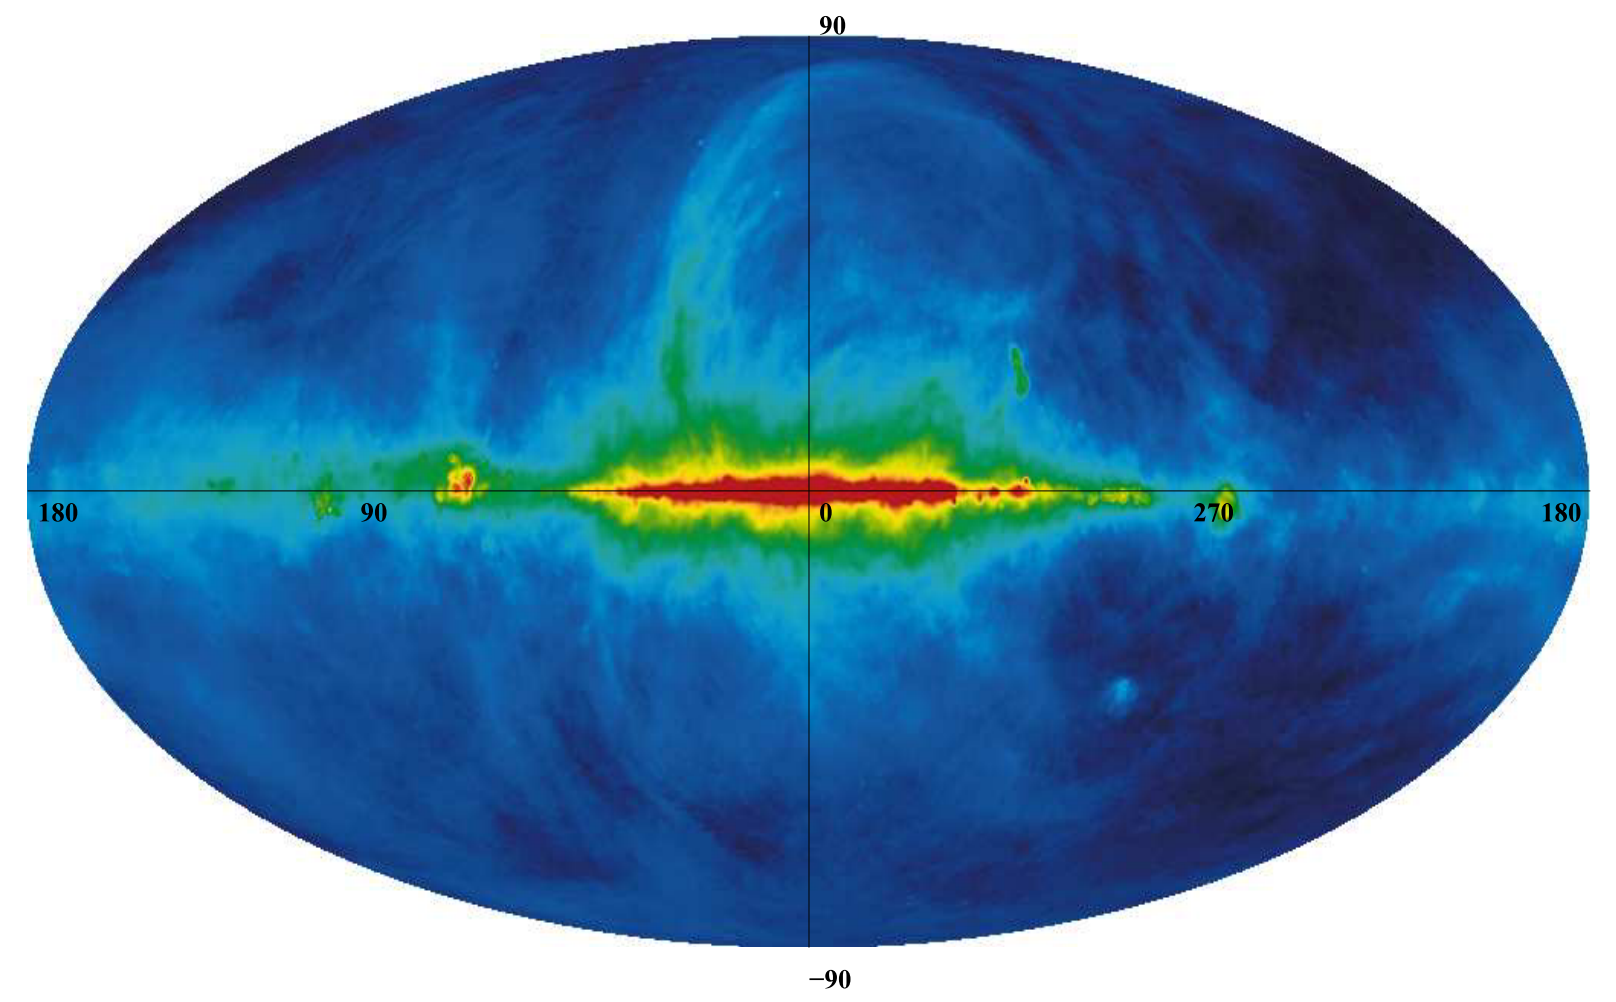
\includegraphics[width=12cm]{figures/Haslam408.png}
    \caption{\footnotesize{The synchrotron emission at $408\,{\rm MHz}$ across the entire sky in Galactic coordinates. As expected the emission is concentrated along the Galactic plane. The noticeable feature known as Loop I is clearly arching up from $\ell=55^\circ$ towards the North Galactic Pole. This figure is adapted from Haslam et al. (1981). Figure taken from Newton-McGee (2009).}}
    \label{fig:haslam408}
\end{figure}

{\noindent}\textbf{Cosmic rays} (i.e., high energy nuclei and electrons) are an important component of the ISM along with magnetic fields and interstellar gas. While the origin of cosmic rays is still not comprehensively understood, it is believed that the electrons with an energy approaching $100-1000\,{\rm TeV}$ have been accelerated in SNRs, suggesting this is one mechanism for the primary formation of cosmic rays.

{\noindent}Magnetic fields accelerate these charged particles via the \textbf{Lorentz force}. The acceleration is given by

\begin{align*}
    \frac{{\rm d}}{{\rm d}\tau}(m\gamma v) = q\left(\frac{\vec{v}}{c}\times\vec{B}\right) ~ [{\rm N}]
\end{align*}

{\noindent}where $m$ is the mass of the particle with charge $q$, $\tau$ is the retarded time, the Lorentz factor  $\gamma=(1 v^2/c^2)^{-1/2}$, and $\vec{B}$ is the magnetic field. The trajectory of the particle is \textit{helical}, with a \textbf{gyration frequency} $\omega_B$ and \textbf{pitch angle} $\theta$ (where $\theta=90^\circ$ for a circular orbit, and $\theta=0^\circ$ for a particle trajectory parallel to $\vec{B}$).

\begin{figure}[h]
    \floatbox[{\capbeside\thisfloatsetup{capbesideposition={right,top},capbesidewidth=4cm}}]{figure}[\FBwidth]
    {\caption{\footnotesize{\\The trajectory of a relativistic electron spiraling in a magnetic field B with a pitch angle $\theta$. The electric field $E$ is polarized parallel to the orbital plane. The synchrotron emission is emitted in a highly beamed cone. This figure is adapted from Kraus (1986). Figure taken from Newton-McGee (2009).}}
    \label{fig:synchrotrondiagram}}
    {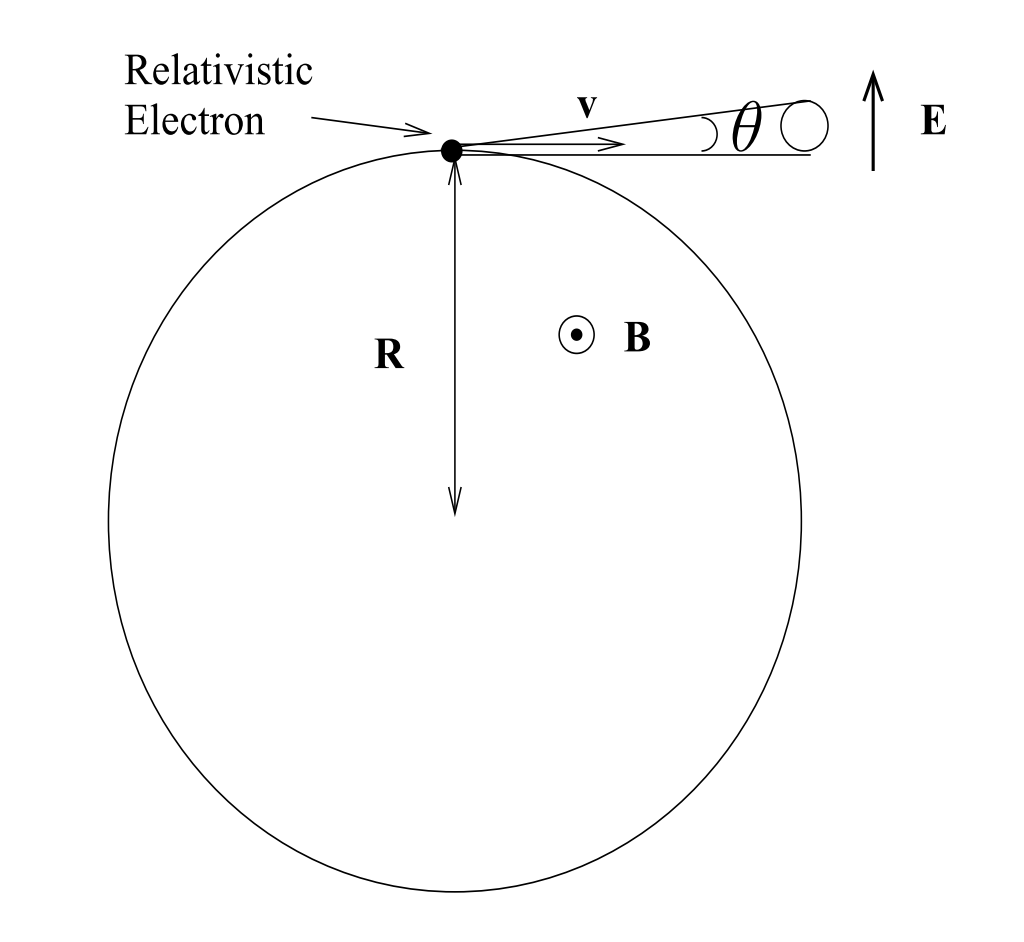
\includegraphics[width=6cm]{figures/SynchrotronDiagram.png}}
\end{figure}

{\noindent}A charged particle deflected by magnetic fields while moving at relativistic speeds emits synchrotron radiation during this acceleration. The main properties of the synchrotron radiation are the following:

\begin{itemize}
    \item high intensity;
    \item very broad and continuous spectral range from infrared up to the hard x-ray region;
    \item natural narrow angular collimation;
    \item high degree of polarization;
    \item pulsed time structure.
\end{itemize}

The graphical representation of synchrotron radiation, depicted in Figure \ref{fig:synchrotrondiagram}, shows that the velocity vector of the particle generates the surface of a cone, with the synchrotron emission beamed within the surface of the cone, at an angle of:

\begin{align*}
    \theta = \pm \frac{mc^2}{E} ~ [{\rm rad}].
\end{align*}

{\noindent}On the surface of the cone the radiation is $100\%$ linearly polarized with its electric field in the direction $-\vec{v}\times\vec{B}$, where $v$ is the direction of propagation of the electron. The degree of linear polarization, called the polarization fraction $p$, is independent of frequency and depends on the spectral index of the cosmic ray electrons:

\begin{align*}
    p(\alpha) = \frac{3-3\alpha}{5-3\alpha} ~ [{\rm dimensionless}].
\end{align*}

{\noindent}In order to understand the angular and spectral distribution of the emitted radiation of synchrotron radiation, let us remind ourselves of the emission from a classical electron moving at a speed $v$ much lower than the speed of light ($v\ll c$). In this case the emitted pattern is similar to that of an oscillating dipole with its maximum of intensity in the direction perpendicular to the acceleration and does not depend on the electron speed. For a relativistic effect, when the speed of the emitting electrons increases to relativistic values ($v\approx c$) the radiation pattern is compressed into a narrow cone in the direction of motion, resulting into an emission tangential to the particle orbit. The vertical half-opening angle $\theta$ is given by

\begin{align*}
    \theta \approx \frac{mc^2}{E} \approx \frac{1}{\gamma} ~ [{\rm rad}].
\end{align*}

{\noindent}See Figure \ref{fig:synchrotronorbits}.

\begin{figure}[h]
    \centering
    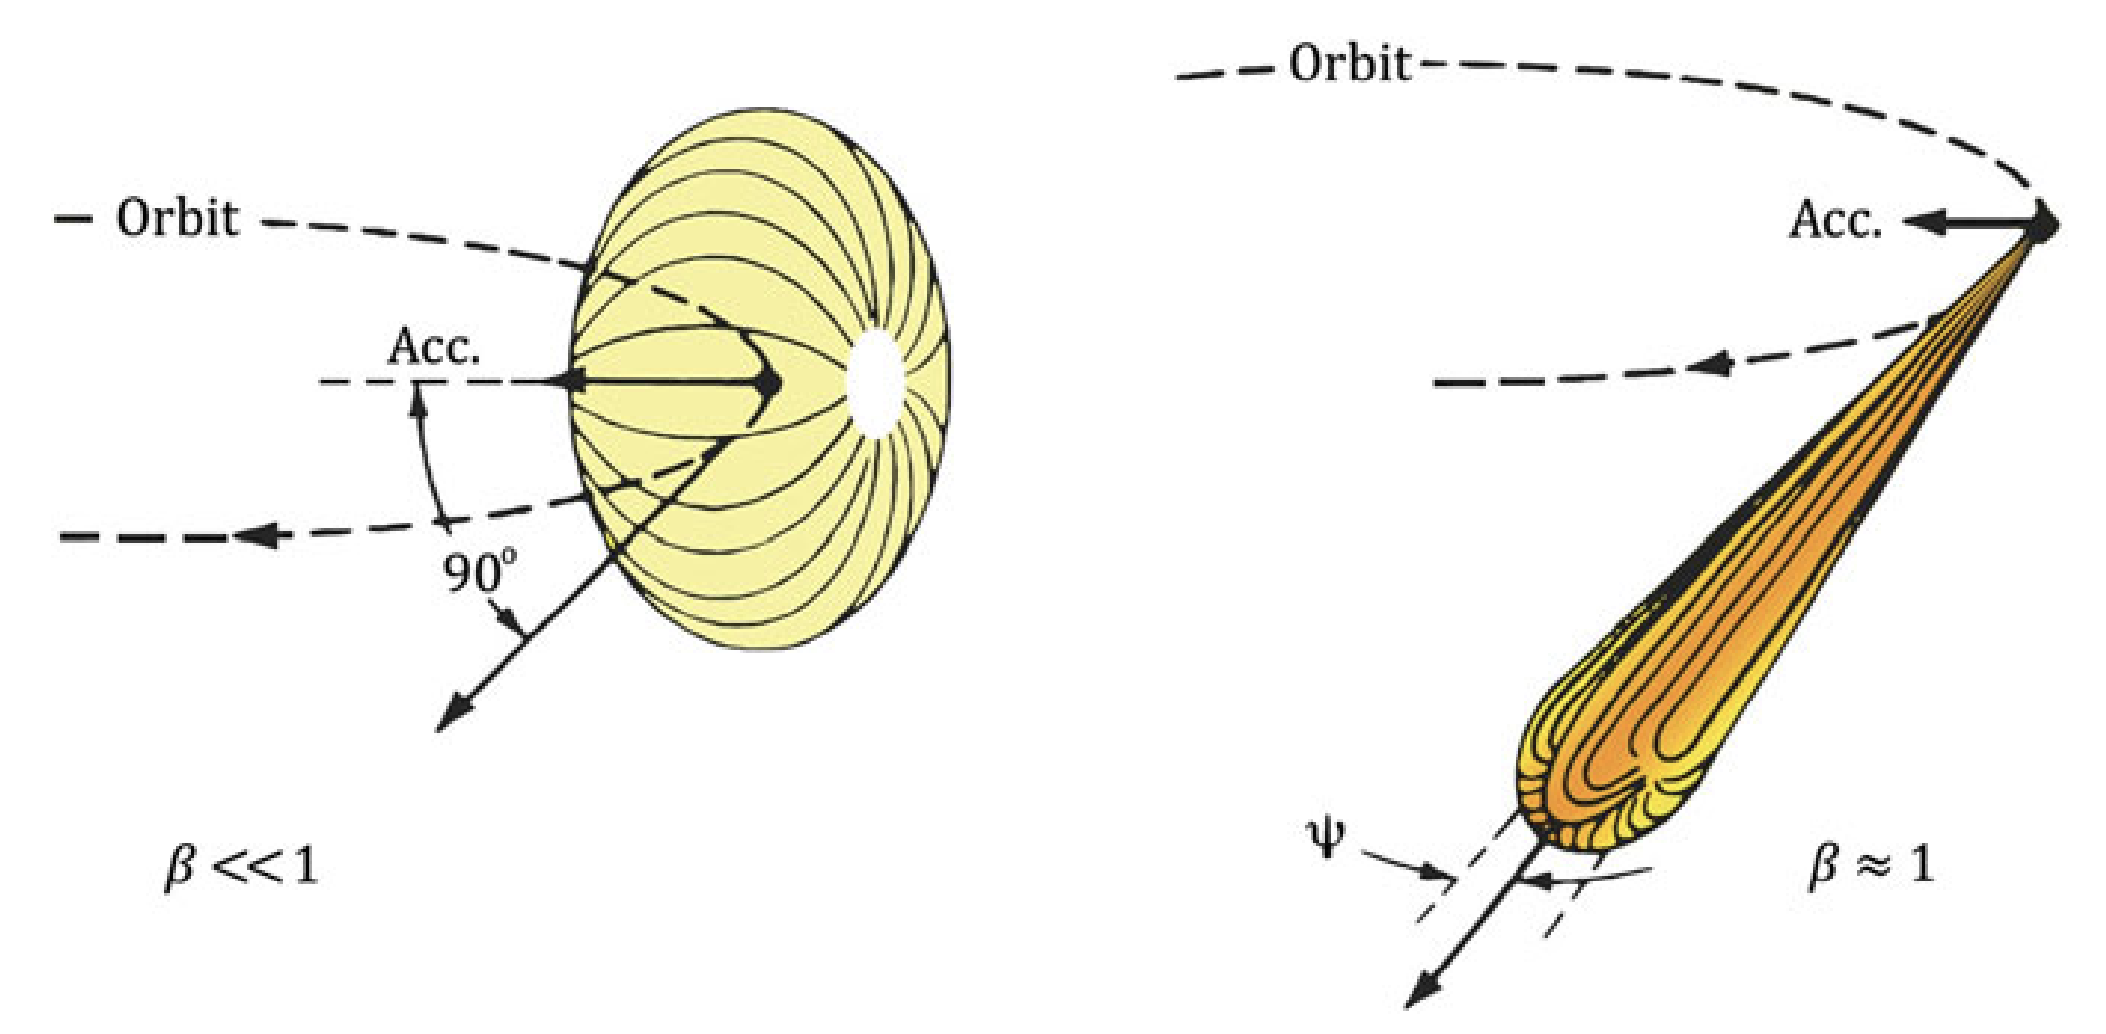
\includegraphics[width=12cm]{figures/SynchrotronOrbits.png}
    \caption{\footnotesize{Qualitative radiation patterns related to charged particles moving in a circular orbit. The dipole pattern is achieved for slow particles when $v/c\ll1$ (left); this is distorted into a narrow cone when $v/c\approx1$ (right). Figure taken from Mobilio et al. (2015).}}
    \label{fig:synchrotronorbits}
\end{figure}

{\noindent}The radiated power from the accelerating charge is given (in cgs units) by

\begin{align*}
    P = \frac{2}{3}\frac{q^4}{m^2c^5} (\gamma\nu)^2 (B\sin\theta)^2 = 2.37\times10^{-15} \left(\frac{E}{{\rm erg}}\right)^2 \left(\frac{B\sin\theta}{\mu{\rm G}}\right)^2 ~ [{\rm erg\,s^{-1}}]
\end{align*}

{\noindent}where the final equality is given for electrons in particular, since the dependence on the mass-to-charge ratio means that electrons are by several orders of magnitude dominant over protons or ions in generating synchrotron radiation. The synchrotron power peaks at the \textbf{characteristic frequency} (in Hz) of

\begin{align*}
    \nu_c = \frac{3}{4\pi}\frac{q}{mc}\gamma^2(B\sin\theta) = 6.26\times10^3 \left(\frac{E}{{\rm erg}}\right)^2 \left(\frac{B\sin\theta}{\mu{\rm G}}\right) ~ [{\rm Hz}].
\end{align*}

{\noindent}This equation tells us that for radio observations (frequencies at or above tens of ${\rm MHz}$) and with typical magnetic field strengths of order $\mu{\rm G}$, the observed population of electrons have $\gamma\gg1$. The radiation is thus highly beamed (width $\sim\gamma^{-1}$) in the direction of the velocity vector. The population of electrons has a power-law energy distribution given by

\begin{align*}
    n(\gamma){\rm d}\gamma = n_0\gamma^{-p}{\rm d}\gamma ~ [{\rm eV^{-1}}]
\end{align*}

{\noindent}where a typical value for the power law index is $p\approx2.5$. The resulting synchrotron luminosity is thus also a power law,

\begin{align*}
    L_\nu \propto \nu^{-(p-1)/2}\equiv \nu^{-\alpha} ~ [{\rm erg\,s^{-1}}]
\end{align*}

{\noindent}with a typical spectral index $\alpha=0.75$ for $p=2.5$. The particles lose energy due to the power emitted with a characteristic timescale of

\begin{align*}
    \tau_{\rm syn} = \frac{\gamma}{{\rm d}\gamma/{\rm d}\tau} = 4\pi\frac{mc}{\sigma_T}\gamma^{-1}(B\sin\theta)^{-2} ~ [{\rm yr}]
\end{align*}

{\noindent}where the \textbf{Thomson cross-section} $\sigma_T=8\pi q^4/3m^2c^4$. Since $\tau_{\rm syn}$ is shorter for more energetic electrons (higher $\gamma$) the power law in the number density $n(\gamma){\rm d}\gamma$ steepens with time (often corresponding to distance from the site of cosmic ray acceleration), therefore increasing the value of $\alpha$. This is referred to as \textbf{synchrotron aging}. Substituting for the characteristic synchrotron frequency $\nu_c$, we can see that

\begin{align*}
    \left(\frac{\tau_{\rm syn}}{{\rm yr}}\right) = 1.06\times10^9 \left(\frac{B\sin\theta}{\mu{\rm G}}\right)^{-1.5} \left(\frac{\nu_c}{{\rm GHz}}\right)^{-0.5}.
\end{align*}

{\noindent}The spectrum of synchrotron radiation must be related to the detailed variation of the electric field as seen by an observer. Because of beaming effects the emitted radiation fields appear to be concentrated in a narrow set of directions about the particle's velocity. The observer will see a pulse of radiation confined to a time interval much smaller than the gyration period. The spectrum will thus be spread over a much broader region than one of order $\omega_B/2\pi$. This is an essential feature of synchrotron radiation.

{\noindent}Non-thermal cosmic radio emission was first thought to originate in stellar atmospheres (the \textbf{radio star hypothesis}). This hypothesis seemed quite reasonable at first glance in view of the existence of quite intense sporadic radio emission from the Sun. It is easy to see, however, that to explain the observed data, these hypothetical radio stars would need to possess extremely unusual properties. The discovery of a quasi-spherical component of the general galactic radio emission imposed severe demands on the radio star hypothesis. For instance, it became clear in this connection that sources of non-thermal galactic radio emission were distributed principally in the galactic halo, the discovery of which had been made only a short time before. Nevertheless, the radio star hypothesis was still not abandoned. If, on the other hand, we equate the general galactic radio emission with synchrotron radiation we then obtain completely probable and useful estimates of the intensity of interstellar fields and the concentration of relativistic electrons. Such estimates are also encouraging in the case of discrete sources. The radio star hypothesis was thus abandoned as early as the beginning of 1953 and the synchrotron character of the major part of non-thermal cosmic radio emission was accepted. 

% --------------------------------------------------------------
%               5. 
% --------------------------------------------------------------

\newpage
\subsection{Question 5}

What are ``forbidden lines'' of atomic spectra? In what conditions are they observationally important? In what conditions do they control the temperature of interstellar material?

\subsubsection{Short answer}

Answer.

\subsubsection{Additional context}

{\noindent}\textbf{Brief overview of atomic structure:} Atoms consist of three subatomic particles: protons, neutrons, and electrons. A proton has a positive charge and a neutron has no charge. Both protons and neutrons are found in the densely packed, positively charged nucleus. The nucleus contains essentially all of the mass of the atom. Electrons carry a negative charge and are found in electron shells surrounding the nucleus. The mass of the electron is considered to be negligible.

{\noindent}All atoms have an atomic number, $Z$, and a mass number, $A$. The atomic number, $Z$, represents its number of protons and its mass number, $A$, represents its number of protons plus its number of neutrons. All atoms of a particular element will have the same atomic number, however they may differ in their number of neutrons and electrons. Two atoms with the same atomic number but different mass numbers (different numbers of neutrons) are referred to as \textbf{isotopes}. The average atomic mass found on the periodic table represents a weighted average of the naturally occurring isotopes for a particular element. Atoms with unequal numbers of protons and electrons produce charged atoms or \textbf{ions}.

{\noindent}Electrons within an atom are found in particular \textbf{orbitals}. An atomic orbital is a mathematical function that describes the wave-like behavior of either one electron or a pair of electrons in an atom. This function can be used to calculate the probability of finding any electron of an atom in any specific region around the atom's nucleus. The term atomic orbital may also refer to the physical region or space where the electron can be calculated to be present, as defined by the particular mathematical form of the orbital. 

{\noindent}Electrons within an atom can be assessed according to the shell, subshell, and orbital to which they are assigned. These assessments are based on the quantum mechanical model. \textbf{Shells} are numbered as $n=1$, $2$, $3$, $4$, etc. and increase in size and energy as they get further away from the nucleus. Shells can be subdivided into subshells.

{\noindent}The maximum number of \textbf{subshells} is equivalent to the shell number. For example, when $n=1$ (first shell), only one subshell is possible and when $n=2$ (second shell), two subshells are possible. There are four different types of subshells. These various types of subshells are denoted by the letters $s$, $p$, $d$, and $f$. Each subshell has a maximum number of electrons which it can hold: $s$: $2$ electrons, $p$: $6$ electrons, $d$: $10$ electrons, and $f$: $14$ electrons. The $s$ subshell is the lowest energy subshell and the $f$ subshell is the highest energy subshell. As was mentioned previously, the shell number is equal to the possible number of subshells. Thus, when $n=1$, the only subshell possible is the $1s$ subshell. When $n=2$, two subshells are possible: the $2s$ and $2p$. When $n=3$, three subshells are possible: the $3s$, $3p$, and $3d$. This means that in the first shell only two electrons are possible and they would be found in the $1s$ ($2$ electrons) subshell. In the second shell, $8$ electrons are possible and would be found in the $2s$ ($2$ electrons) and the $2p$ ($6$ electrons) subshells.

{\noindent}Each subshell is further divided into \textbf{orbitals}. An orbital is defined as a region of space in which an electron can be found. \textit{Only two electrons are possible per orbital}. Thus, the $s$ subshell may contain only one orbital and the $p$ subshell may contain three orbitals. Each orbital has its own distinct shape. An $s$ orbital found in an $s$ subshell is spherical, $p$ orbitals found in $p$ subshells are two-lobed, and $d$ orbitals found in $d$ subshells are four-lobed. Since there are three possible orbitals per $p$ subshell, each orbital adopts its own orientation. The $p_x$ orbital lies along the $x$ axis, the $p_y$ orbital lies along the $y$ axis, and the $p_z$ orbital lies along the $z$ axis.

\begin{figure}[t]
    \centering
    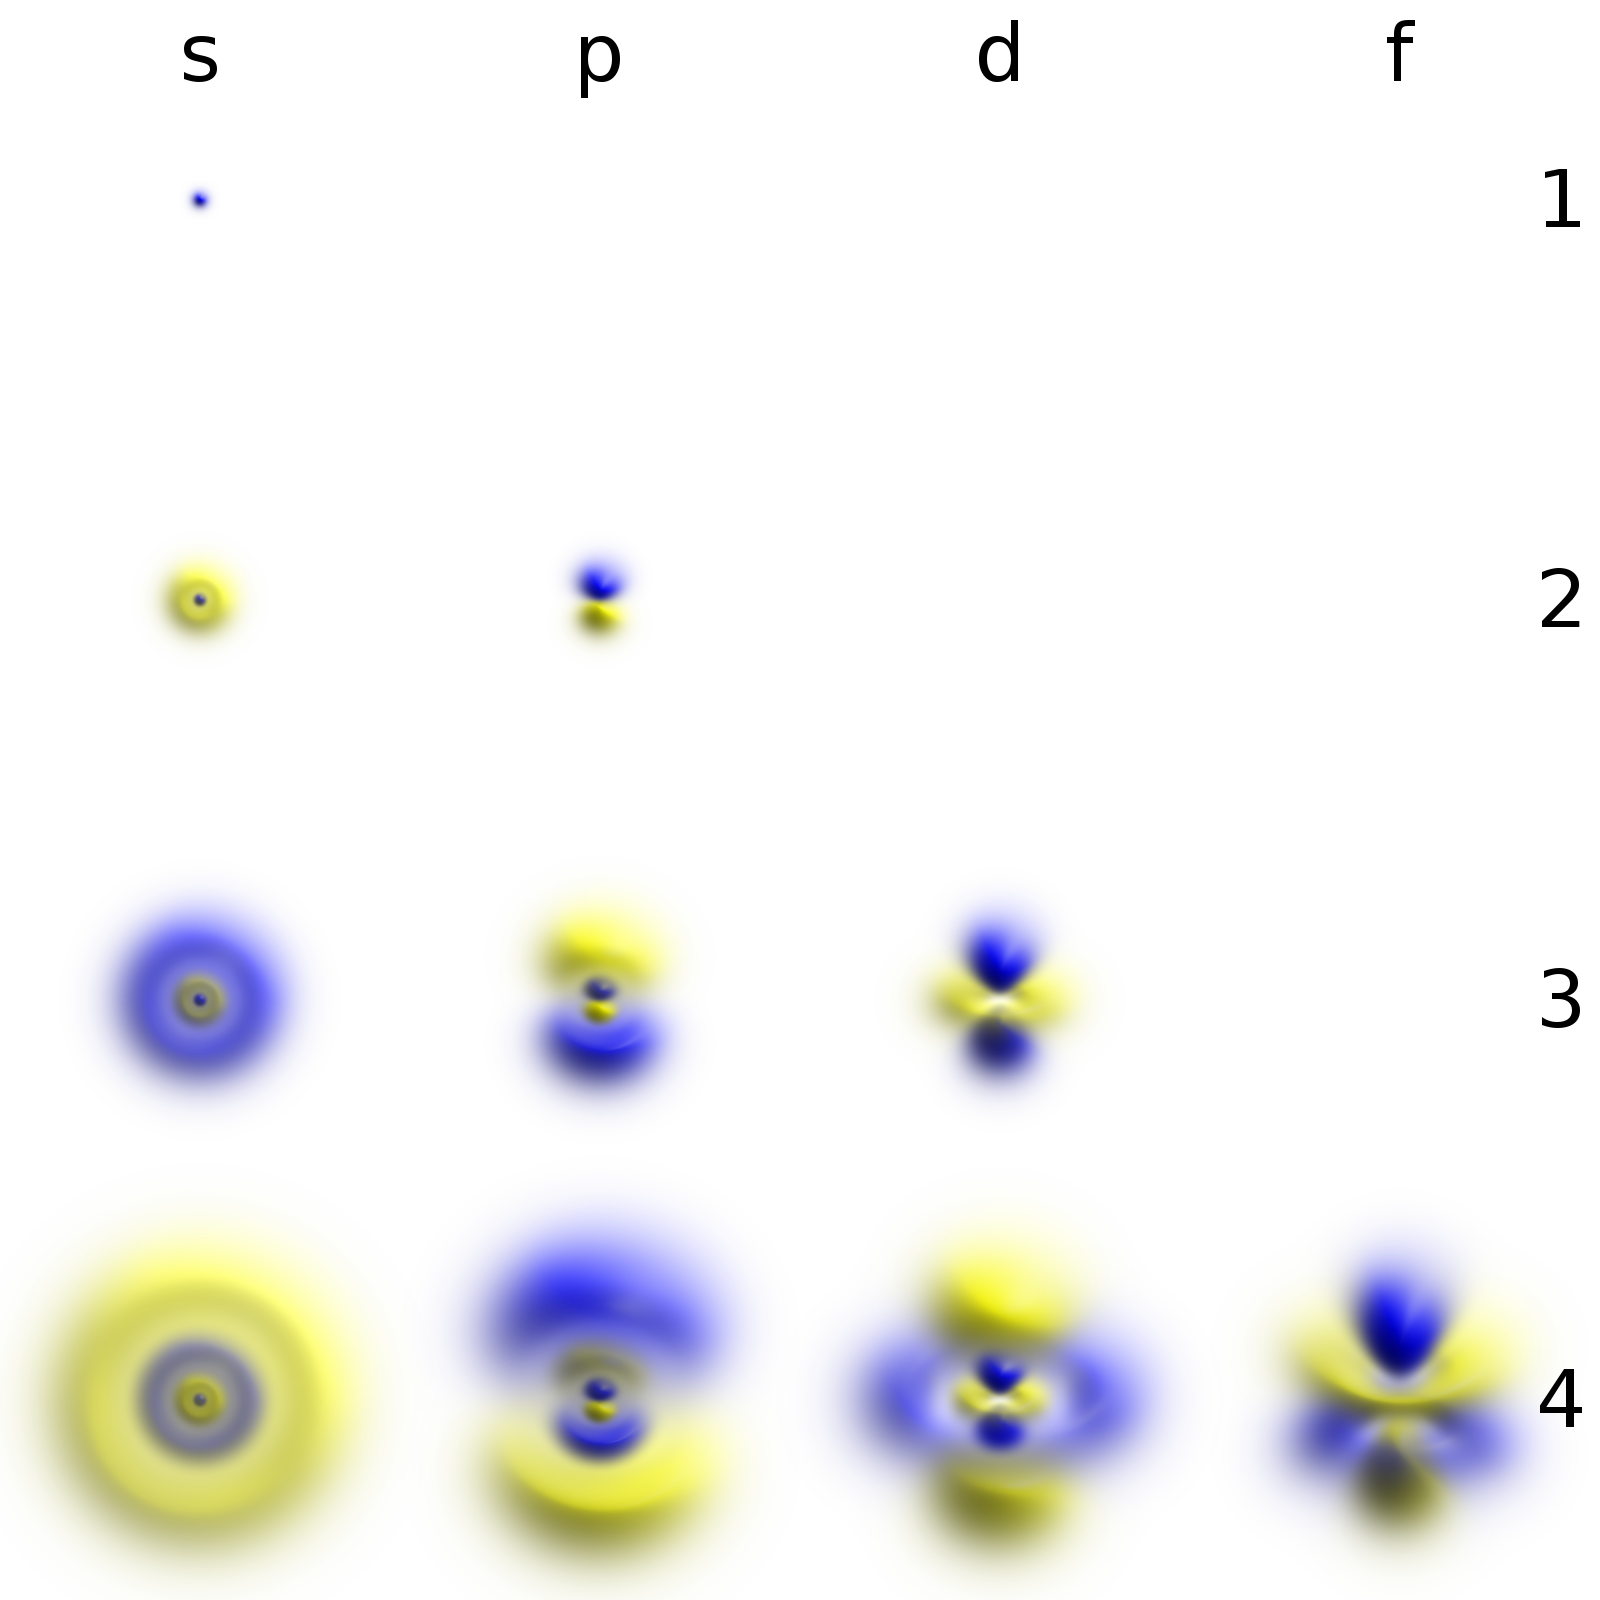
\includegraphics[width=11cm]{figures/orbitals_3D.png}
    \caption{\footnotesize{3D views of some hydrogen-like atomic orbitals. Figure taken from Wikipedia.}}
    \label{fig:orbitals3D}
\end{figure}

{\noindent}When writing electron configurations for atoms, the shorthand symbol for a subshell followed by a super-scripted number which represents the number of electrons in that subshell is used. For example, a Carbon atom with $6$ electrons would have the electron configuration: $1s^22s^22p^2$. A possible arrangement within the $2p$ subshell would be to find one of the electrons in the $2p_x$ orbital and the second electron in the $2p_y$ orbital. 

{\noindent}Figure \ref{fig:orbitals3D} shows hydrogen-like atomic structure for $s$, $p$, $d$, and $f$ orbitals.

{\noindent}\textbf{Selection rules for radiative transitions:} Some energy levels are connected by strong radiative transitions; in other cases, radiative transitions between the levels may be extremely slow. The strong transitions always satisfy what are referred to as the \textbf{selection rules for electric dipole transitions}. Here, we summarize the selection rules for the strong electric dipole transitions, and we also give the selection rules for \textbf{inter-system} and \textbf{forbidden transitions} that do not satisfy the electric dipole selection rules but nevertheless are strong enough to be astrophysically important. We will use the ion NII as an example; the first nine energy levels of NII are shown in Figure \ref{fig:NIIlevels}.

\begin{figure}[t]
    \centering
    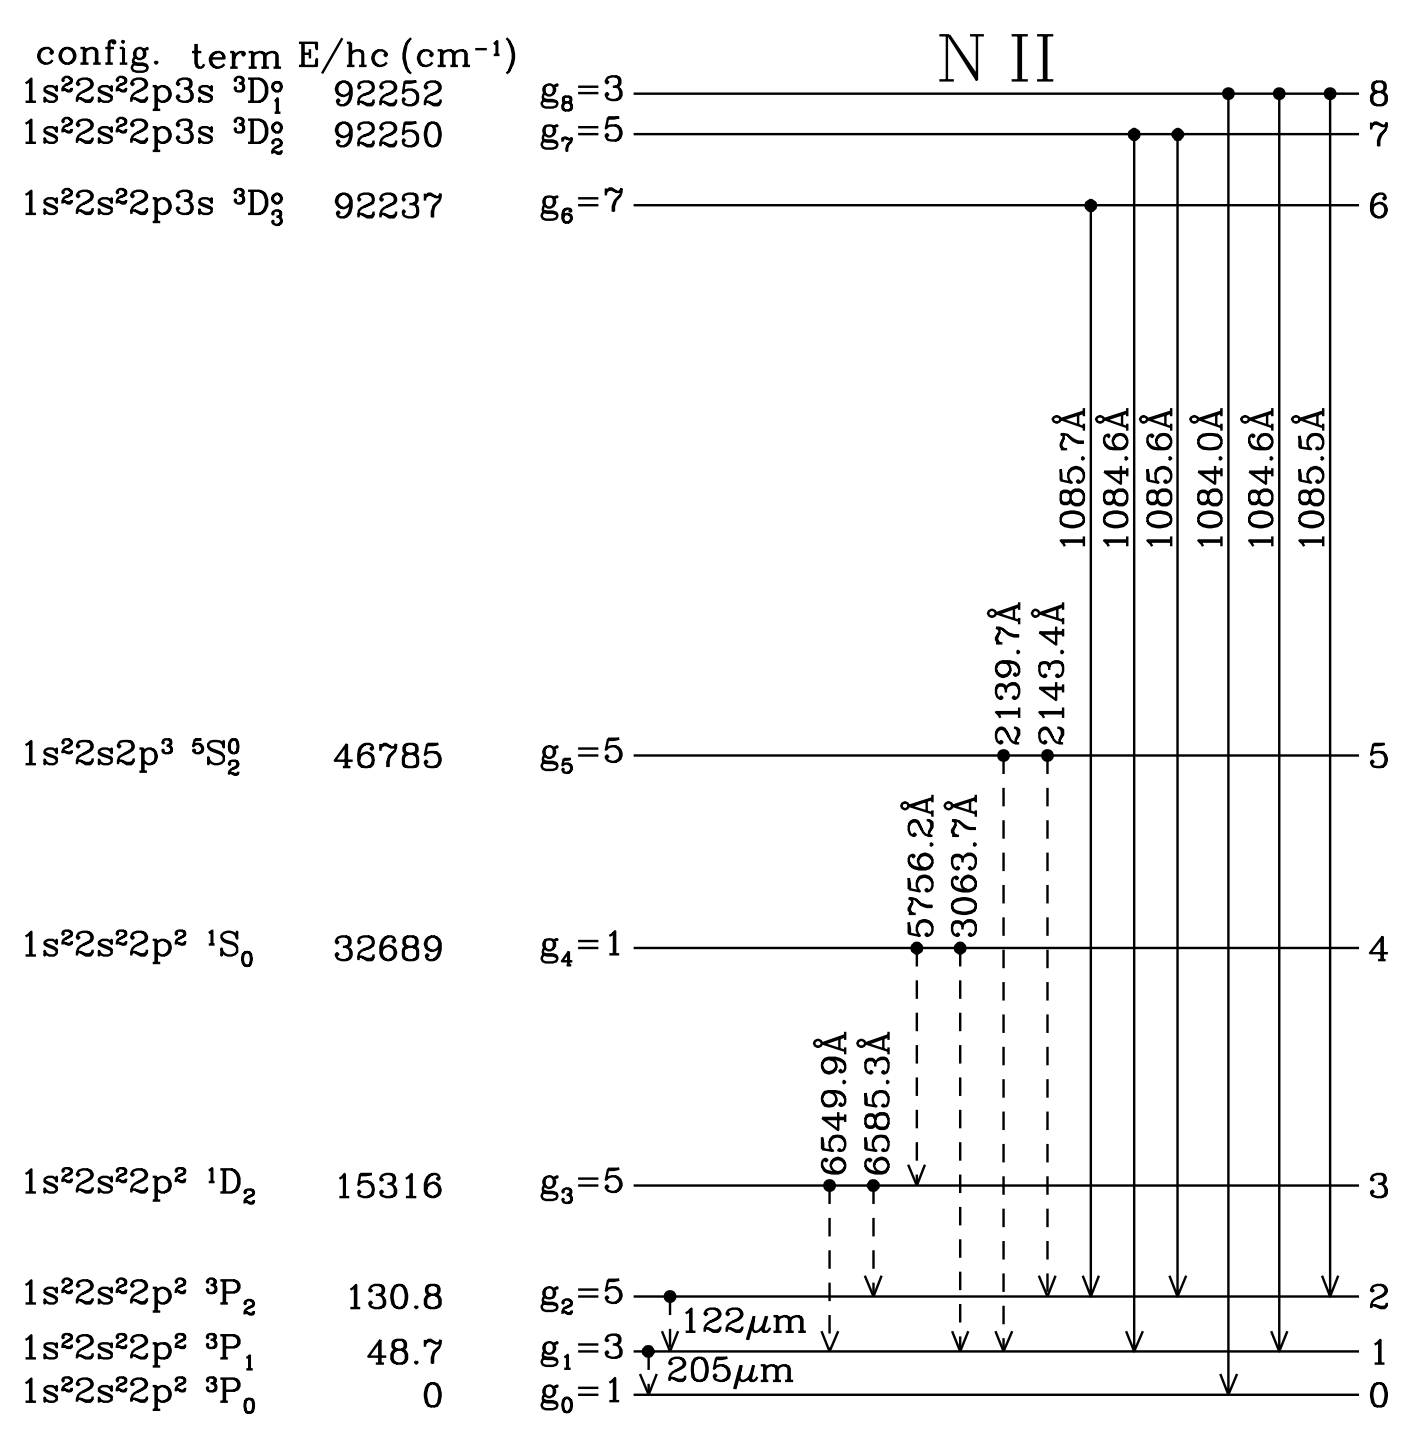
\includegraphics[width=14cm]{figures/NII_levels.png}
    \caption{\footnotesize{First nine energy levels of NII. Forbidden transitions are indicated by broken lines, and allowed transitions by solid lines; forbidden decays are not shown from levels that have permitted decay channels. Fine-structure splitting is not to scale. Hyperfine splitting is not shown. Figure taken from Draine (2015).}}
    \label{fig:NIIlevels}
\end{figure}

{\noindent}\textbf{Allowed: Electric dipole transitions:} The strongest transitions are electric dipole transitions. These are transitions satisfying the following selection rules:

\begin{enumerate}
    \item Parity must change.
    \item $\Delta L = 0, \pm1$.
    \item $\Delta J = 0, \pm1$, but $\Delta J = 0\rightarrow0$ is forbidden.
    \item Only one single-electron wave function $n\ell$ changes, with $\Delta\ell=\pm1$.
    \item $\Delta S=0$: Spin does not change.
\end{enumerate}

{\noindent}An allowed transition is denoted \textit{without} square brackets, for example,

\begin{align*}
    {\rm NII}\,1084.0{\rm \AA}\,^3P_0-^3D_1^o.
\end{align*}

{\noindent}This is a transition between the $\ell=1s^22s^22p^2\,3P_0$ and $u=1s^22s^22p3s\,^3D_1^o$ levels of NII, with a wavelength $\lambda_{u\ell}=1084.0$\,\AA. The transition has $A_{u\ell}=2.18\times10^8\,{s^{-1}}$. This decay is very fast -- the lifetime of the $^3D_1^o$ level against this decay is only $1/A_{u\ell}=4.6\,{\rm ns}$!

{\noindent}\textbf{Spin-Forbidden or inter-system transitions:} These are transitions that fulfill the electric dipole selection rules $1$ to $4$ but have $\Delta S\neq0$. These transitions are considerably weaker than allowed transitions. Such transitions are sometimes referred to as \textbf{semi-forbidden}, or \textbf{inter-combination}, or \textbf{inter-system transitions}; the latter is the terminology that we will use. An inter-system transition is denoted with a single right bracket -- for example,

\begin{align*}
    {\rm NII]}\,2143.4{\rm \AA}\,^3P_2-^5S_2^o.
\end{align*}

{\noindent}This is a transition between the $\ell=1s^22s^22p^2\,3P_2$ and $u=1s^22s2p^3\,^5S_2^o$ levels of NII, with a wavelength $\lambda_{u\ell}=2143.4$\,\AA\,and $A_{u\ell}=1.27\times10^2\,{\rm s^{-1}}$.

{\noindent}\textbf{Forbidden transitions:} Forbidden transitions are those that fail to fulfill at least one of the selection rules $1$ to $4$. The transition probabilities vary widely, depending on the values of the electric quadrupole or magnetic dipole matrix elements between the upper and lower states. A forbidden transition is denoted with two square brackets -- for example,

\begin{align*}
    {\rm [NII]}\,6549.9{\rm \AA}\,^3P_1-^1D_2^o.
\end{align*}

{\noindent}This is a transition between the $\ell=1s^22s^22p^2\,3P_1$ and $u=1s^22s^22p^2\,^1D_2^o$ levels of NII, with a wavelength $\lambda_{u\ell}=6549.9$\,\AA\,and $A_{u\ell}=9.20\times10^{-4}\,{\rm s^{-1}}$. This fails rule $1$ (parity is unchanged) and it fails rule $4$ (single electron wave functions are unchanged). This is an example of a \textbf{magnetic dipole transition}.

{\noindent}Another example of a forbidden transition is the \textbf{electric quadrupole transition}

\begin{align*}
    {\rm [NII]}\,5756.2{\rm \AA}\,^1D_2-^1S_0^o.
\end{align*}

{\noindent}This is a transition between the $\ell=1s^22s^22p^2\,1D_2$ and $u=1s^22s^22p^2\,^1S_0^o$ levels of NII, with a wavelength $\lambda_{u\ell}=5756.2$\,\AA\,and $A_{u\ell}=1.17\,{\rm s^{-1}}$. This fails rules $1$ (parity is unchanged) and $4$ (single electron wave functions are unchanged) and it fails rules $2$ and $3$ ($\Delta L=-2$ and $\Delta J=-2$), yet its transition probability is three orders of magnitude larger than the magnetic dipole transition [NII]\,$6549.9$\AA!

{\noindent}We see then that there is a hierarchy in the transition probabilities: very roughly speaking, inter-system lines are $\sim10^6$ times weaker than permitted transitions, and forbidden lines are $\sim10^2-10^6$ times weaker than inter-system transitions.

{\noindent}Despite being very ``weak,'' forbidden transitions are important in astrophysics for the simple reason that every atom and ion has excited states that can only decay via forbidden transitions. At high densities, such excited states would be depopulated by collisions, but at the very low densities of interstellar space, collisions are sufficiently infrequent that there is time for forbidden radiative transitions to take place.

\subsubsection{Follow-up Questions}

\begin{itemize}
    \item What are some common examples of forbidden lines?
    \item When do you get forbidden line absorption?
    \item What kind of radiation can be absorbed by forbidden line absorption?
    \item Can we observe any forbidden lines on Earth?
    \item What is the lifetime of the 21 cm line?
    \item At what redshifts do CMB photons get absorbed by 21 cm transitions?
    \item At what redshifts do you get neutral hydrogen?
    \item How would you estimate the lifetime from the maximum density where the line isn't washed out?
    \item Collisions happen much more frequently; why is the 21 cm line still visible?
    \item Why does forbidden line emission cool the gas?
    \item Why are they \textit{so good} at cooling the gas?
\end{itemize}

% --------------------------------------------------------------
%               6. 
% --------------------------------------------------------------

\newpage
\subsection{Question 6}

What is a polytropic equation of state? Give examples of objects for which this is a very good approximation, and explain why it is.

\subsubsection{Short answer}

Answer.

\subsubsection{Additional context}

{\noindent}\textbf{Eulerian description}: For gaseous, non-rotating, single stars without strong magnetic fields, the only forces acting on a mass element come from pressure and gravity. This results in a spherically symmetric configuration. All functions will then be constant on concentric spheres, and we need only one spatial variable to describe them. It seems natural to use the distance r from the stellar centre as the spatial coordinate, which varies from r D 0 at the centre to the total radius r D R at the surface of the star. In addition, the evolution in time t requires a dependence of all functions on t: If we thus take r and t as independent variables, we have a typical ``Eulerian'' treatment in the sense of classical hydrodynamics. Then all other variables are considered to depend on these two, for example, the density $\rho=\rho(r,t)$.

{\noindent}\textbf{Lagrangian description}: It will turn out that, in the spherically symmetric case, it is often more useful to take a ``Lagrangian'' coordinate instead of r (i.e., one which is connected to the mass elements). The spatial coordinate of a given mass element then does not vary in time. We choose for this coordinate the above defined $m$: to any mass element, the value $m$ (which is the mass contained in a concentric sphere at a given moment $t_0$) is assigned once and for all.

{\noindent}The new independent variables are then $m$ and $t$; and all other variables are considered to depend on them; for example, $\rho=\rho(m,t)$. This also includes the radial distance $r$ of our mass element from the centre, which is now described by the function $r=r(m,t)$. Since there is certainly no singularity of $\rho$ at the centre, we have here $m=0$, while the star's total mass $m=M$ is reached at the surface (i.e., where $r=R$). This already shows one advantage of the new description for the (normal) case of stars with constant total mass: while the radius $R$ varies strongly in time, the star always extends over the same interval of the independent variable $m:0\leq m \leq M$. Although real stars do lose mass, for example, by stellar winds or due to gravitational interaction in binary systems, over short timescales the assumption of constant mass is justified nevertheless. In any case, the range of $m$ never changes by more than a factor of a few.

{\noindent}As just indicated, there will certainly be no problem concerning a unique one-to-one transformation between the two coordinates $r$ and $m$: We then easily find the connection between the partial derivatives in the two cases from well-known formulae. For any function depending on two variables, one of which is substituted by a new one ($r,t\rightarrow m,t$), the partial derivatives with respect to the new variables are given by

\begin{align*}
    \frac{\partial}{\partial m} &= \frac{\partial}{\partial r} \cdot \frac{\partial r}{\partial m} \\
    \left(\frac{\partial}{\partial t}\right)_m &= \frac{\partial}{\partial r}\cdot \left(\frac{\partial r}{\partial t}\right)_m + \left(\frac{\partial}{\partial t}\right)_r.
\end{align*}

{\noindent}Subscripts indicate which of the spatial variables ($m$ or $r$) is considered constant. The second of these equations reveals the main reason for the choice of the Lagrangian description. Its left-hand side gives the so-called \textbf{substantial time derivative} of hydrodynamics. It describes the change of a function in time when following a given mass element (e.g., the change of a physical property of this mass element). The conservation laws for time-dependent spherical stars give very simple equations only in terms of this substantial time derivative. In terms of a local time derivative, $(\partial/\partial t)_r$, the description would become much more complicated since the ``convective'' terms with the velocity $(\partial r/\partial t)_m$ would appear explicitly.

{\noindent}Let us apply the first of these to $m$. We know that $m$ varies with $r$ as

\begin{align*}
    \frac{\partial m}{\partial r} = 4\pi r^2 \rho.
\end{align*}

{\noindent}Taking the partial derivative $\partial/\partial m$, we obtain

\begin{align*}
    \frac{\partial}{\partial m} \left(\partial m\right) &= \frac{\partial}{\partial m} \left(4\pi r^2 \rho\right) \partial r \\
    1& = \frac{\partial r}{\partial m} \left(4\pi r^2 \rho\right) \\
    \frac{\partial r}{\partial m} &= \frac{1}{4\pi r^2 \rho}.
\end{align*}

{\noindent}This is a differential equation describing the spatial behaviour of the function $r(m,t)$. It replaces $\partial m/\partial r=4\pi r^2\rho$ in the Lagrangian description. Introducing this differential equation into the partial differential equation we just found for $\partial/\partial m$, we find the general recipe for the transformation between the two operators:

\begin{align*}
    \frac{\partial}{\partial m} = \frac{1}{4\pi r^2\rho} \frac{\partial}{\partial r}.
\end{align*}

{\noindent}In the deep interiors of stars the gases are fully ionized (i.e., for each hydrogen nucleus there also exists a free electron, while for each helium nucleus there are two free electrons). We therefore have a mixture of two gases, that of the nuclei (which in itself can consist of more than one component) and that of the free electrons. The mixture can be treated similarly to a one-component gas, if all single components obey the ideal gas law.

{\noindent}Let's consider a mixture of fully ionized nuclei. The chemical composition can be described by specifying all $X_i$ ; the weight fractions of nuclei of type $i$ which have molecular weight $\mu_i$ and charge number $Z_i$. If we have $n_i$ nuclei per volume and a ``partial density'' $\rho_i$, then $X_i=\rho_i/\rho$ and

\begin{align*}
    n_i = \frac{\rho_i}{\mu_im_{\rm H}} = \frac{\rho}{m_{\rm H}} \frac{X_i}{\rho_i}.
\end{align*}

{\noindent}By $L_r$ we define the net energy per second passing outward through a sphere of radius $r$. The function $L_r$ is zero at $r=0$, since there can be no infinite energy source at the centre, while $L_r$ reaches the total luminosity $L$ of the star at the surface. In between, $L_r$ can be a complicated function, depending on the distribution of the sources and sinks of energy.

{\noindent}The function $L_r$ comprises the energies transported by radiation, conduction, and convection. Not included is a possible energy flux by neutrinos, which normally have negligible interaction with the stellar matter. Also included in $L_r$ are only those fluxes which require a temperature gradient.

{\noindent}Consider a spherical mass shell of radius $r$; thickness ${\rm d}r$; and mass ${\rm d}m$. The energy per second entering the shell at the inner surface is $L_r$, while $L_r+{\rm d}L_r$ is the energy per second leaving it through the outer surface. The surplus power ${\rm d}L_r$ can be provided by nuclear reactions, by cooling, or by compression or expansion of the mass shell.

{\noindent}We first consider a stationary case in which ${\rm d}L_r$ is due to the release of energy from nuclear reactions only. Let $\epsilon$ be the \textbf{nuclear energy produced per gram of stellar material}; then

\begin{align*}
    {\rm d}L_r &= 4\pi r^2\rho\epsilon{\rm d}r = \epsilon {\rm d}m \\
    \frac{{\rm d}L_r}{{\rm d}m} &= \epsilon ~ [{\rm eV\,g^{-1}}].
\end{align*}

{\noindent}In general $\epsilon$ depends on the temperature and density, and on the abundance of the different nuclear species that react.

{\noindent}Let us denote the types of reacting particles, $X$ and $a$, by indices $j$ and $k$ respectively. Suppose there is one particle of type $j$ moving with a velocity $v$ relative to all particles of type $k$. Its cross section $\sigma$ for reactions with $k$ sweeps over a volume $\sigma v$ per second. The number of reactions per second will then be $n_k \sigma v$ if there are $n_k$ particles of type $k$ per unit volume. For $n_j$ particles per unit volume the total number of reactions per units of volume and time is

\begin{align*}
    \tilde{r}_{jk} = n_jn_k\sigma v.
\end{align*}

{\noindent}This product may also be interpreted by saying that $n_jn_k$ is the number of pairs of possible reaction partners, and $\sigma v$ gives the reaction probability per pair and second. This indicates what we have to do in the case of reactions between identical particles ($j=k$). Then the number of pairs that are possible reaction partners is $n_j(n_j-1)/2\approx n_j^2/2$ for large particle numbers. This has to replace the product $n_jn_k$ so that we can generally write

\begin{align*}
    \tilde{r}_{jk} = \frac{1}{1+\delta_{jk}}n_jn_k\sigma v
\end{align*}

{\noindent}\textbf{The full set of equations}: Collecting the basic differential equations for a spherically symmetric star in hydrostatic equilibrium, we obtain a full set of differential equations that describe stellar evolution:

\begin{equation*}
\boxed{
    \begin{aligned}
        \frac{\partial r}{\partial m} &= \frac{1}{4\pi r^2\rho} \\
        \frac{\partial P}{\partial r} &= -\frac{GM_r}{4\pi r^4} \\
        \frac{\partial L}{\partial m} &= \epsilon_n-\epsilon_\nu-c_P \frac{\partial T}{\partial t} + \frac{\delta}{\rho}\frac{\partial P}{\partial t} \\
        \frac{\partial T}{\partial m} &= -\frac{GM_rT}{4\pi r^4P}\nabla \\
        \frac{\partial X_i}{\partial t} &= \frac{m_i}{\rho} \left(\sum_jj_{ji} - \sum_kr_{ik}\right), ~~~ i=1,...,I.
    \end{aligned}
}
\end{equation*}

{\noindent}The second equation has an additional term $-\partial^2r/\partial t^2(4\pi r^2)^{-1}$ in case the assumption of hydrostatic equilibrium is not fulfilled. In the last equation, we have a set of $I$ equations (one of which may be replaced by the normalization $\sum_iX_i=1$) for the change of mass fractions $X_i$ of the relevant nuclei $i=1,..,I$ having masses $m_i$. In the third equation, $\delta\equiv-(\partial\ln\rho/\partial\ln T)_P$, and in the second last equation $\nabla\equiv{\rm d}\ln T/{\rm d}\ln P$. If the energy transport is due to radiation (and conduction), then $\nabla$ has to be replaced by $\nabla_{\rm rad}$ given by 

\begin{align*}
    \nabla_{\rm rad} = \frac{3}{16\pi acG}\frac{\kappa LP}{mT^4} ~ [{\rm K\,P^{-1}}].
\end{align*}

{\noindent}If the energy is carried by convection, then $\nabla$ has to be replaced by a value obtained from a proper theory of convection; this may be $\nabla_{\rm ad}$ in the deep interior given by 

\begin{align*}
    \nabla_{\rm ad} = \left(1-\frac{1}{\gamma}\right) \frac{\mu m_{\rm H}}{k}\frac{GM_r}{r^2} ~ [{\rm K\,m^{-1}}],
\end{align*}

{\noindent}or one obtained from a solution of the cubic equation for super-adiabatic convection in the outer layers.

{\noindent}The boxed equations contain functions which describe properties of the stellar material such as $\rho, \epsilon_n, \epsilon_\nu,\kappa,c_P,$ and the reaction rates $r_{ij}$. We shall assume them to be known functions of $P, T$, and the chemical composition described by the functions $X_i(m,t)$ We therefore have an equation of state

\begin{align*}
    \rho = \rho(P,T,X_i) ~ [{\rm g\,cm^{-3}}],
\end{align*}

{\noindent}and equations for the other thermodynamic properties of the stellar matter

\begin{align*}
    c_P &= c_P (P,T,X_i) \\
    \delta &= \delta (P,T,X_i) \\
    \nabla_{\rm ad} &= \nabla_{\rm ad} (P,T,X_i),
\end{align*}

{\noindent}as well as the Rosseland mean of the opacity (including conduction)

\begin{align*}
    \kappa = \kappa (P,T,X_i),
\end{align*}

{\noindent}and the nuclear reaction rates and the energy production and energy loss via neutrinos:

\begin{align*}
    r_{jk} &= r_{jk} (P,T,X_i) \\
    \epsilon_\nu &= \epsilon_\nu (P,T,X_i) \\
    \epsilon_\nu &= \epsilon_\nu (P,T,X_i).
\end{align*}

{\noindent}\textbf{Polytropic equations}: The temperature does not appear explicitly in the first two boxed equations. Under certain circumstances this provides the possibility of separating them from the ``thermo-energetic part'' of the equations. For the following it is convenient to introduce the gravitational potential $\Phi$. We here treat stars in hydrostatic equilibrium, which requires

\begin{align*}
    \frac{{\rm d}P}{{\rm d}r} = - \frac{{\rm d}\Phi}{{\rm d}r} \rho,
\end{align*}

{\noindent}together with Poisson's equation

\begin{align*}
    \frac{1}{r^2}\frac{{\rm d}}{{\rm d}r} \left(r^2\frac{{\rm d}\Phi}{{\rm d}r}\right) = 4\pi G\rho.
\end{align*}

{\noindent}We have replaced the partial derivatives by ordinary ones since only time-independent solutions shall be considered.

{\noindent}In general the temperature appears in these equations if the density is replaced by an equation of state of the form $\rho=\rho(P,T)$. However, if $\rho$ does not depend on $T$ (i.e., $\rho=\rho(P)$), then this relation can be introduced, which become a system of two equations for $P$ and $\Phi$ and can be solved without the other structure equations. An example is the completely degenerate gas of non-relativistic electrons for which $\rho\sim P^{3/5}$.

{\noindent}We shall deal here with similar cases and assume that there exists a simple relation between $P$ and $\rho$ of the form

\begin{align*}
    P = K\rho^\gamma \equiv K\rho^{1+1/n} ~ [{\rm P}],
\end{align*}

{\noindent}where $K$, $\gamma$, and $n$ are constants. A relation of this form is called a \textbf{polytropic equation of state}. $K$ is the \textbf{polytropic constant} and $\gamma$ is the \textbf{polytropic exponent} (which we have to distinguish from the adiabatic exponent $\gamma_{\rm ad}$). One often uses, instead of $\gamma$, the \textbf{polytropic index} $n$, which is defined by

\begin{align*}
    n = \frac{1}{\gamma-1} ~ [{\rm dimensionless}].
\end{align*}

{\noindent}For a completely degenerate gas the equation of state in its limiting cases has the polytropic form as seen above. In the non-relativistic limit we have $\gamma=5/3$, $n=3/2$, while for the relativistic limit $\gamma=4/3$, $n=3$. For such cases, where the equation of state has a polytropic form, the polytropic constant $K$ is fixed and can be calculated from natural constants. There are also examples of the polytropic equation of state where $K$ is a free parameter which is constant within a particular star but can have different values from one star to another.

{\noindent}In a star that is completely convective the temperature gradient (except for that in a region near the surface, which we shall ignore) is given, to a very good approximation, by $\nabla=({\rm d}\ln T/{\rm d}\ln P)_{\rm ad}=\nabla_{ad}$. If radiation pressure can be ignored and the gas is completely ionized, we have $\nabla_{\rm ad}=2/5$. This means that throughout the star $T\sim P^{2/5}$, and for an ideal gas with $\mu={\rm constant}$, $T\sim P/\rho$, and therefore $P\sim\rho^{5/3}$. This again is a polytropic relation with  $\gamma=5/3$, $n=3/2$. But now $K$ is not fixed by natural constants; it is a free parameter in the sense that it can vary from star to star.

{\noindent}The homogeneous gaseous sphere can also be considered a special case of the polytropic relation. Let us write the polytropic equation of state in the form

\begin{align*}
    \rho = K_1P^{1/\gamma} ~ [{\rm g\,cm^{-3}}].
\end{align*}

{\noindent}Then $\gamma=\infty$ (or $n=0$) gives $\rho=K_1={\rm constant}$.

{\noindent}These examples have shown that we can have two reasons for a polytropic relation in a star:
\begin{enumerate}
    \item The equation of state is of the simple form $P=K\rho$ with a fixed value of $K$;
    \item The equation of state contains $T$ (as for an ideal gas), but there is an additional relation between $T$ and $P$ (like the adiabatic condition) that together with the equation of state yields a polytropic relation; then $K$ is a free parameter.
\end{enumerate}

{\noindent}On the other hand, if we assume a polytropic relation for an ideal gas, this is equivalent to adopting a certain relation $T=T(P)$. This means that one fixes the temperature stratification instead of determining it by the thermo-energetic equations of stellar structure. For example, a polytrope with $n=3$ does not necessarily have to consist of relativistic degenerate gases but can also consist of an ideal gas and have $\nabla=1/(n+1)=0.25$.

{\noindent}\textbf{Polytropic stellar models}: With the polytropic relation (independent of whether $K$ is a free parameter or a constant with a fixed value), the equation of hydrostatic equilibrium can be written as

\begin{align*}
    \frac{{\rm d}\Phi}{{\rm d}r} = -\gamma K\rho^{\gamma-2} \frac{{\rm d}\rho}{{\rm d}r}.
\end{align*}

{\noindent}If $\gamma\neq1$ (the case $\gamma=1, n=\infty$ corresponding to the isothermal model, this can be integrated:

\begin{align*}
    \rho = \left( \frac{-\Phi}{(n+1)K} \right)^n ~ [{\rm g\,cm^{-3}}],
\end{align*}

{\noindent}where we have made use of $n=1/(\gamma-1)$ and chosen the integration constant to give $\Phi=0$ at the surface ($\rho=0$). Note that in the interior of our model, $\Phi<0$, giving there $\rho>0$. If we introduce this form of $\rho$ into the right-hand side of the Poisson equation, we obtain an ordinary differential equation for $\Phi$:

\begin{align*}
    \frac{{\rm d}^2\Phi}{{\rm d}r^2} + \frac{2}{r}\frac{{\rm d}\Phi}{{\rm d}r} = 4\pi G \left( \frac{-\Phi}{(n+1)K} \right)^n.
\end{align*}

{\noindent}We now define dimensionless variables $z$, $w$ by

\begin{align*}
    z &= Ar ~ [{\rm dimensionless}], ~~~ A^2 = \frac{4\pi G}{(n+1)^nK^n}(-\Phi^c)^{n-1} = \frac{4\pi G}{(n+1)K}\rho_c^{(n-1)/n} ~ [{\rm dimensionless}],\\
    w &= \frac{\Phi}{\Phi_c} = \left(\frac{\rho}{\rho_c}\right)^{1/n} ~ [{\rm dimensionless}],
\end{align*}

{\noindent}where the subscript $c$ refers to the centre and where the relation between $\rho$ and $\Phi$ is taken from $\rho=[-\Phi/(n+1)K]^n$. At the centre ($r=0$) we have $z=0, \Phi=\Phi_c, \rho=\rho_c$, and therefore $w=1$. Then the ordinary differential equation for $\Phi$ can be written as

\begin{align*}
    \frac{{\rm d}^2w}{{\rm d}z^2} +\frac{2}{z}\frac{{\rm d}w}{{\rm d}z} + w^n &= 0 \\
    \frac{1}{z^2}\frac{{\rm d}}{{\rm d}z} \left(z^2 \frac{{\rm d}w}{{\rm d}z}\right) + w^n &= 0.
\end{align*}

{\noindent}This is the famous \textbf{Lane-Emden equation} (named after J.H. Lane and R. Emden). We are only interested in solutions that are finite at the centre, $z=0$. This equation shows that we then have to require ${\rm d}w/{\rm d}z\equiv w'=0$. Let us assume we have a solution $w(z)$ of the Lane-Emden equation that fulfills the central boundary conditions $w(0)=1$ and $w'(0)=0$; then according to the definition of $w$ the radial distribution of the density is given by

\begin{align*}
    \rho(r) = \rho_cw^n ~ [{\rm g\,cm^{-3}}], ~~~ \rho_c = \left[ \frac{-\Phi_c}{(n+1)K} \right]^n ~ [{\rm g\,cm^{-3}}].
\end{align*}

{\noindent}For the pressure we obtain from the polytropic equation that $P(r)=P_cw^{n+1}$, where $P_c=K\rho_c^\gamma$.

% --------------------------------------------------------------
%               7. 
% --------------------------------------------------------------

\newpage
\subsection{Question 7}

What was the solar neutrino problem, and how was it resolved?

\subsubsection{Short answer}

Answer.

\subsubsection{Additional context}

{\noindent}\textbf{Solar neutrinos:} Some of the nuclear reactions of the pp chain, as well as of the CNO cycle, produce neutrinos. In addition, there are also neutrinos due to the very rare \textit{pep} and \textit{hep} reactions

\begin{align*}
    {\rm ^1H+^1H+e^- \rightarrow\,^2H+\nu\,(\textit{pep})} \\
    {\rm ^3He+^1H \rightarrow\,^4He+e^++\nu\,(\textit{hep})},
\end{align*}

{\noindent}the latter one being the trivial way to produce $^4$He after the \textbf{pp-chain},

\begin{align*}
    {\rm ^1H+^1H \rightarrow\,^2H+e^++\nu,} \\
    {\rm ^2H+^1H \rightarrow \,^3He+\gamma},
\end{align*}

{\noindent}but it is occurring in only $10^{-8}$ of all cases. However, the energy of the emitted neutrino is close to $10\,{\rm MeV}$, and it is therefore necessary to consider this reaction. The neutrinos leave the star practically without interacting with the stellar matter. The energy spectrum of neutrinos from $\beta$ decay is continuous, since the electrons can take part of the energy away, while neutrinos released after an inverse $\beta$ decay are essentially monochromatic. Therefore most reactions of the pp chain have a continuous spectrum, while the pep-reaction and the electron capture on $^7$Be have a line spectrum. Since $^7$Be can decay into $^7$Li either in the ground state or in an excited state, this reaction gives two spectral lines. The neutrino spectrum of the Sun as predicted from the reactions of the pp chain, computed from our standard solar model, is given in Figure \ref{fig:neutrinospectrum}.

{\noindent}Since the solar neutrinos can leave the Sun almost unimpeded they can in principle be measured in terrestrial laboratories and thus be used to learn directly about conditions in the innermost solar core. This difficult task indeed has been undertaken since 1964, when John Bahcall and Raymond Davies began to plan for an underground neutrino detector in a mine in Homestead, North Dakota. Forty years later the experiments finally have confirmed the standard solar model, and R. Davies received the Nobel Prize for his work. The time in between, however, was characterized by the \textbf{solar neutrino problem}.

{\noindent}The solar neutrino problem consisted in the fact that since the first results from the so-called chlorine experiment by Davies there was a lack of neutrinos compared to solar model predictions. The chlorine experiment is sensitive to neutrinos with energies above $0.814\,{\rm MeV}$ and therefore, as can be seen in Figure \ref{fig:neutrinospectrum} mainly to the $^8$B neutrinos, with some contribution from pep, hep, and $^7$Be neutrinos. The experiment is based on the reaction $^{37}{\rm Cl}+\nu\rightarrow\,^{37}{\rm Ar}$, where the decays of radioactive argon nuclei are counted. The rate of neutrino captures is commonly measured in solar neutrino units (SNU). One SNU corresponds to $10^{-36}$ captures per second and per target nucleus. The predicted counts amount to $7.5\,{\rm SNU}$ for the chlorine experiment, the measurements averaged over several decades to only $2.5\pm0.2\,{\rm SNU}$. The deficit could indicate that the solar centre is cooler than in the models.

{\noindent}To improve the experimental evidence, additional experiments were started. First, another kind of radio-chemical detector using gallium in the detector fluid measured, due to a much lower energy threshold, the majority of neutrinos, including those from the pp-reaction. Later, electron-scattering detectors were developed, which are sensitive to the highest energies only, but which provide directional information about the neutrino source (for these detectors the \textit{hep}-neutrinos of have to be taken into account.). All experiments confirmed that the solar neutrino flux was of the right order of magnitude, and therefore that indeed the Sun shines by the nuclear fusion of hydrogen, but they also consistently measured a deficit of neutrinos. This deficit, however, varied between different kinds of detectors.

{\noindent}With more and more experimental data it became evident that even hypothetical changes to the solar centre cannot solve the problem and that the solution is most likely to be found in the properties of neutrinos. All nuclear reactions emit electron neutrinos, and these are the only ones that were measured in terrestrial experiment, with the exception of the electron-scattering Sudbury Neutrino Observatory (SNO) experiment in Canada, where heavy water (with a high percentage of deuterium isotopes) was used as the detector. Here also reactions with the two other types (flavours) of neutrinos, muon and tau neutrinos can be detected. Summing these and the electron neutrinos up, the total number of detections is completely consistent with the solar model prediction, within a few percent. What created the apparent solar neutrino deficit is the fact that neutrinos can change their flavour, both while travelling through vacuum and more efficiently in the presence of electrons in the solar interior. A similar effect was also confirmed for muon neutrinos arising in the Earth's upper atmosphere from high-energy cosmic radiation, when measured before or after they have travelled through the Earth's interior. The modelling of the solar interior, together with sophisticated experiments, has therefore resulted in new knowledge about fundamental properties of neutrinos. In particular, these so-called \textbf{neutrino oscillations} are possible only if neutrinos have mass.

\begin{figure}[t]
    \floatbox[{\capbeside\thisfloatsetup{capbesideposition={right,top},capbesidewidth=4cm}}]{figure}[\FBwidth]
    {\caption{\footnotesize{The neutrino spectrum of the Sun as predicted from the theoretical standard solar model. The solid lines belong to reactions of the pp chain while the broken lines are due to reactions of the CNO cycle. The neutrinos from most of the reactions have continuous spectra, while mono-energetic neutrinos come from $^7$Be and from the pep-reaction. The flux  for the continuum sources is given in $cm^2\,s^{-1}\,MeV^{-1}$ and for the line sources in $cm^2\,s^{-1}$. The sensitivity of the three types of neutrino experiments is indicated above the figure and by the shaded regions. Figure taken from Kippenhahn, Weigert \& Weiss (2012).}}
    \label{fig:neutrinospectrum}}
    {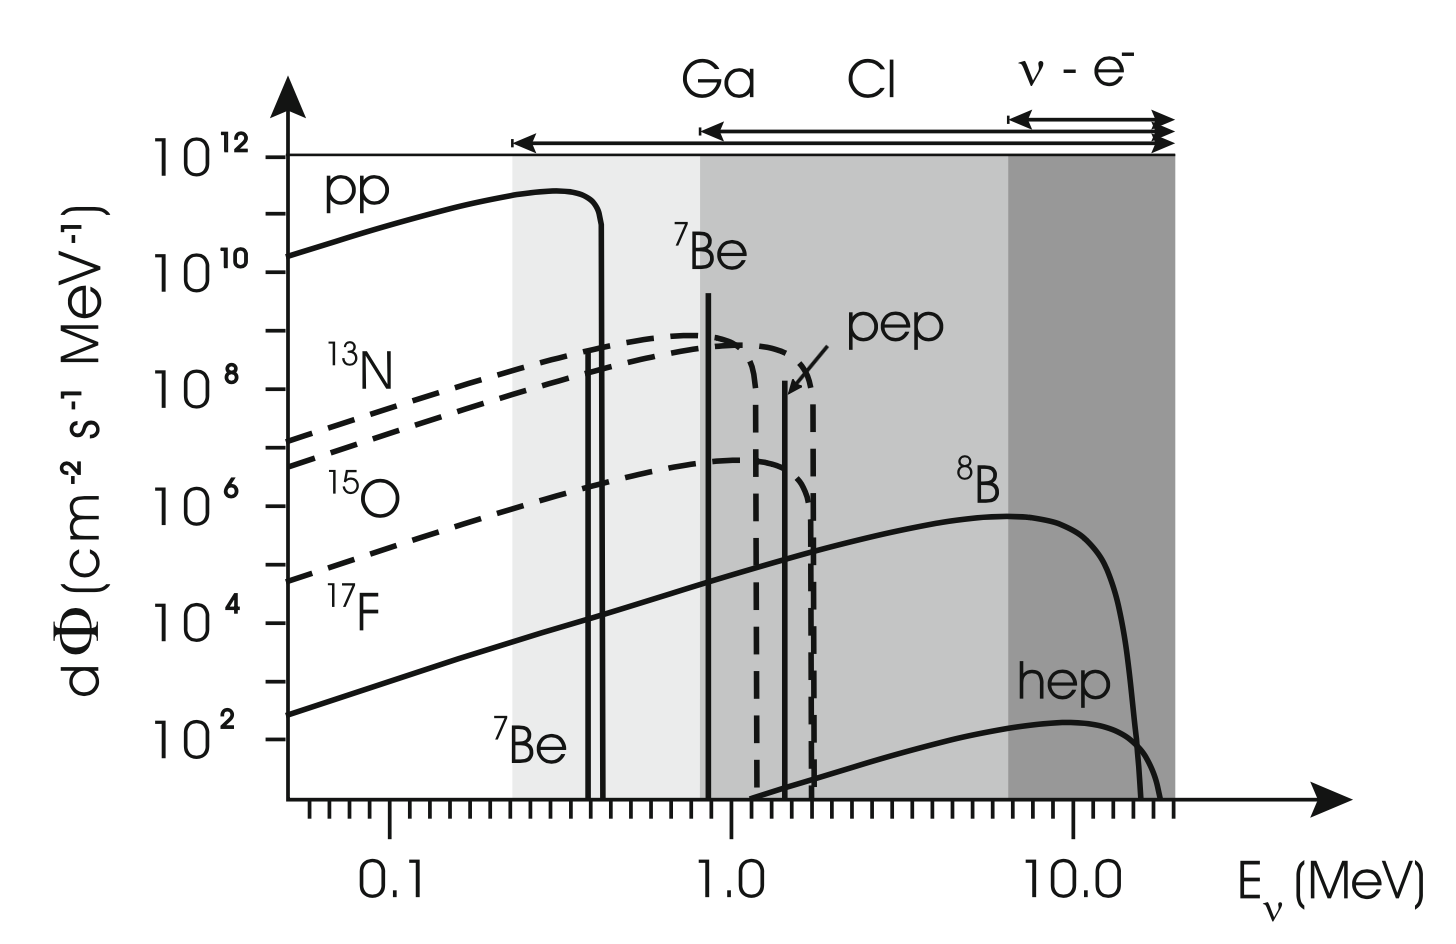
\includegraphics[width=10cm]{figures/NeutrinoSpectrum.png}}
\end{figure}

{\noindent}\textbf{The evolution of neutrino astronomy}: The following is from the brief Millennium Essay for the PASP on the evolution of neutrino astronomy from the personal perspective of John Bahcall and Raymon Davis, Jr (2000).

{\noindent}The possibility of observing solar neutrinos began to be discussed seriously following the 1958 experimental discovery by H. P. Holmgren and R. Johnston that the cross section for production of the isotope $^7$Be by the fusion reaction $^3{\rm He}+^4{\rm He}\rightarrow^7{\rm Be}+\gamma$ was more than a thousand times larger than was previously believed. This result led Willy Fowler and Al Cameron to suggest that $^8$B might be produced in the Sun in sufficient quantities by the reaction $^7{\rm Be}+p\rightarrow^8{\rm B}+\gamma$ to produce an observable flux of high energy neutrinos from $^8$B beta-decay.

{\noindent}We begin our story in 1964, when we published back-to-back papers in Physical Review Letters arguing that a 100,000 gallon detector of perchloroethylene could be built which would measure the Solar neutrino capture rate on chlorine. Our motivation was to use neutrinos to look into the interior of the Sun and thereby test directly the theory of stellar evolution and nuclear energy generation in stars. The particular development that made us realize that the experiment could be done was the theoretical discovery (by John in late 1963) that the principal neutrino absorption cross section on chlorine was 20 times larger than previously estimated due to a super-allowed nuclear transition to an excited state of argon.

{\noindent}If you have a good idea today, it likely will require many committees, many years, and many people in order to get the project from concept to observation. The situation was very different in 1964. Once the decision to go ahead was made, a very small team designed and built the experiment; the entire team consisted of Ray, Don Harmer (on leave from Georgia Tech), and John Galvin (a technician who worked part-time on the experiment). Kenneth Hoffman, a (then) young engineer, provided expert advice on technical questions. The money came out of the chemistry budget at Brookhaven National Laboratory. Neither of us remember a formal proposal ever being written to a funding agency. The total capital expenditure to excavate the cavity in the Homestake Gold Mine in South Dakota, to build the tank, and to purchase the liquid was \$0.6 million dollars (in 1965 dollars).

{\noindent}During the period 1964-1967, Fred Reines and his group worked on three Solar neutrino experiments in which recoil electrons produced by neutrino interactions would be detected by observing the associated light in an organic scintillator. Two of the experiments, which exploited the elastic scattering of neutrinos by electrons, were actually performed and led to a (higher than predicted) upper limit on the $^8$B solar neutrino flux. The third experiment, which was planned to detect neutrinos absorbed by $^7$Li, was abandoned after the initial chlorine results showed that the solar neutrino flux was low. These three experiments introduced the technology of organic scintillators into the arena of Solar neutrino research, a technique that will only finally be used in 2001 when the BOREXINO detector will begin to detect low-energy Solar neutrinos. Also during this period, John investigated the properties of neutrino electron scattering and showed that the forward peaking from $^8$B neutrinos is large, a feature that was incorporated two and half decades later in the Kamiokande (and later Super-Kamiokande) water Cerenkov detectors.

{\noindent}The first results from the chlorine experiment were published in 1968, again in a back-to-back comparison (in Physical Review Letters) between measurements and standard predictions. The initial results have been remarkably robust; the conflict between chlorine measurements and standard Solar model predictions has lasted over three decades. The main improvement has been in the slow reduction of the uncertainties in both the experiment and the theory. The efficiency of the Homestake chlorine experiment was tested by recovering carrier solutions, by producing $^{37}$Ar in the tank with neutron sources, and by recovering $^{36}$Cl inserted in a tank of perchloroethylene. The Solar model was verified by comparison with precise helioseismological measurements.

{\noindent}For much more than two decades, the best estimates for the observational and for the theoretical prediction have remained essentially constant. The discrepancy between the standard Solar model predictions and the chlorine observations became widely known as the \textbf{Solar neutrino problem}. 

{\noindent}Very few people worked on Solar neutrinos during the period 1968-1988. The chlorine experiment was the only solar neutrino experiment to provide data in these two decades. It is not easy for us to explain why this was the cas;; we certainly tried hard to interest others in doing different experiments, and we gave many joint presentations about what came to be known as the solar neutrino problem. Each of us had one principal collaborator during this long period, Bruce Cleveland (experimental) and Roger Ulrich (Solar models). A large effort to develop a chlorine experiment in the Soviet Union was led by George Zatsepin, but it was delayed by the practical difficulties of creating a suitable underground site for the detector. Eventually, the effort was converted into a successful gallium detector, SAGE, led by Vladimir Gavrin and Tom Bowles, that gave its first results in 1990.

{\noindent}Only 1 year after the first (1968) chlorine results were published, Vladimir Gribov and Bruno Pontecorvo proposed that the explanation of the Solar neutrino problem was that neutrinos oscillated between the state in which they were created and a more difficult to detect state. This explanation, which is the consensus view today, was widely disbelieved by nearly all the particle physicists we talked to in those days. In the form in which Solar neutrino oscillations were originally proposed by Gribov and Pontecorvo, the process required that the mixing angles between neutrino states be much larger than the quark mixing angles, something which most theoretical physicists believed, at that time, was unlikely. Ironically, a flood of particle theory papers explained, more or less ``naturally,'' the large neutrino mixing angle that was decisively demonstrated 30 years later in the Super-Kamiokande atmospheric neutrino experiment.

{\noindent}One of the most crucial events for early Solar neutrino research occurred in 1968 while we were relaxing in the Sun after a swim at the Caltech pool. Gordon Garmire (now a PI for the Chandra X-ray Observatory) came up to Ray, introduced himself, and said he had heard about the chlorine experiment. He suggested to Ray that it might be possible to reduce significantly the background by using pulse rise-time discrimination, a technique used for proportional counters in space experiments. The desired fast-rising pulses from $^{37}$Ar Auger electrons are different from the slower rising pulses from a background gamma or cosmic ray. Ray went back to Brookhaven and asked the local electronic experts if it would be possible to implement this technique for the very small counters he used. The initial answer was that the available amplifiers were not fast enough to be used for this purpose with the small Solar neutrino counters. But, in about a year three first-class electronic engineers at Brookhaven, Veljko Radeca, Bob Chase, and Lee Rogers, were able to build electronics fast enough to be used to measure the rise time in Ray's counters.

{\noindent}This ``swimming pool'' improvement was crucial for the success of the chlorine experiment and the subsequent radio-chemical gallium solar neutrino experiments, SAGE, GALLEX, and GNO. Measurements of the rise time as well as the pulse energy greatly reduce the background for radio-chemical experiments. The backgrounds can be as low as one event in 3 months. 

{\noindent}In 1978, after a decade of disagreement between the Homestake neutrino experiment and standard Solar model predictions, it was clear to everyone that the subject had reached an impasse and a new experiment was required. The chlorine experiment is, according to standard Solar model predictions, sensitive primarily to neutrinos from a rare fusion reaction that involves $^8$B neutrinos. These neutrinos are produced in only $2$ of every $10^4$ terminations of the basic p-p fusion chain. In the early part of 1978, there was a conference of interested scientists who got together at Brookhaven to discuss what to do next. The consensus decision was that we needed an experiment that was sensitive to the low-energy neutrinos from the fundamental p-p reaction.

{\noindent}The only remotely practical possibility appeared to be another radio-chemical experiment, this time with $^{71}$Ga (instead of $^{37}$Cl) as the target. But, a gallium experiment (originally proposed by the Russian theorist V. A. Kuzmin in 1965) was expensive; we needed about 3 times the world's annual production of gallium to do a useful experiment. In an effort to generate enthusiasm for a gallium experiment, we wrote another Physical Review Letters paper, this time with a number of interested experimental colleagues. We argued that a gallium detector was feasible and that a gallium measurement, which would be sensitive to the fundamental p-p neutrinos, would distinguish between broad classes of explanations for the discrepancy between prediction and observation in the $^{37}$Cl experiment. Over the next $5$ or $6$ years, the idea was reviewed a number of times in the United States, always very favorably. The Department of Energy (DOE) appointed a blue ribbon panel headed by Glen Seaborg that endorsed enthusiastically both the experimental proposal and the theoretical justification.

{\noindent}To our great frustration and disappointment, the gallium experiment was never funded in the United States, although the experimental ideas that gave rise to the Russian experiment (SAGE) and the German-French-Italian-Israeli-US experiment (GALLEX) originated largely at Brookhaven. Physicists strongly supported the experiment and said the money should come out of the astronomy budget; astronomers said it was great physics and should be supported by the physicists. DOE could not get the nuclear physics and the particle physics sections to agree on who had the financial responsibility for the experiment. In a desperate effort to break the deadlock, John was even the PI of a largely Brookhaven proposal to the National Science Foundation (which did not support proposals from DOE laboratories). A pilot experiment was performed with $1.3$ tons of gallium by an international collaboration (Brookhaven, University of Pennsylvania; Max Planck Institute, Heidelberg; Institute for Advanced Study, Princeton; and the Weizmann Institute) which developed the extraction scheme and the counters eventually used in the GALLEX full-scale experiment.

{\noindent}In strong contrast to what happened in the United States, Moissey Markov, the head of the Nuclear Physics Division of the Russian Academy of Sciences, helped establish a neutrino laboratory within the Institute for Nuclear Research, participated in the founding of the Baksan neutrino observatory, and was instrumental in securing $60$ tons of gallium free to Russian scientists for the duration of a Solar neutrino experiment. The Russian-American gallium experiment (SAGE) went ahead under the leadership of Vladimir Gavrin, George Zatsepin (Institute for Nuclear Research, Russia), and Tom Bowles (Los Alamos), and the mostly European experiment (GALLEX) was led by Till Kirsten (Max Planck Institute, Germany). Both experiments had a strong but not primary US participation.

{\noindent}The two gallium experiments were performed in the decade of the 1990s and gave very similar results, providing the first experimental indication of the presence of p-p neutrinos. Both experiments were tested by measuring the neutrino rate from an intense laboratory radioactive source.

{\noindent}There were two dramatic developments in the Solar neutrino saga, one theoretical and one experimental, before the gallium experiments produced observational results. In 1985, two Russian physicists proposed an imaginative solution of the Solar neutrino problem that built upon the earlier work of Gribov and Pontecorvo and, more directly, the insightful investigation by Lincoln Wolfenstein (of Carnegie Mellon University). Stanislav Mikheyev and Alexei Smirnov showed that if neutrinos have masses in a relatively wide range, then a resonance phenomenon in matter (now universally known as the \textbf{MSW effect}) could convert efficiently many of the electron-type neutrinos created in the interior of the Sun to more difficult to detect muon and tau neutrinos. The MSW effect can work for small or large neutrino mixing angles. Because of the elegance of the theory and the possibility of explaining the experimental results with small mixing angles (analogous to what happens in the quark sector), physicists immediately began to be more sympathetic to particle physics solutions to the Solar neutrino problem. More importantly, they became enthusiasts for new Solar neutrino experiments.

{\noindent}The next big breakthrough also came from an unanticipated direction. The Kamiokande water Cerenkov detector was developed to study proton decay in a mine in the Japanese Alps; it set an important lower limit on the proton lifetime. In the late 1980s, the detector was converted by its Japanese founders, Masatoshi Koshiba and Yoji Totsuka, together with some American colleagues (Gene Beier and Al Mann of the University of Pennsylvania), to be sensitive to the lower energy events expected from Solar neutrinos. With incredible foresight, these experimentalists completed in late 1986 their revisions to make the detector sensitive to Solar neutrinos, just in time to observe the neutrinos from SN 1987a emitted in the LMC 170,000 years earlier. (Supernova and Solar neutrinos have similar energies, $\sim10\,{\rm MeV}$, much less than the energies that are relevant for proton decay.) In 1996, a much larger water Cerenkov detector (with 50,000 tons of pure water) began operating in Japan under the leadership of Yoji Totsuka, Kenzo Nakamura, Yoichiro Suzuki (from Japan), and Jim Stone and Hank Sobel (from the United States).

{\noindent}So far, five experiments have detected solar neutrinos in approximately the numbers (within a factor of $2$ or $3$) and in the energy range ($<15\,{\rm MeV}$) predicted by the standard Solar model. This is a remarkable achievement for Solar theory since the $^8$B neutrinos that are observed primarily in three of these experiments (chlorine, Kamiokande, and its successor Super-Kamiokande) depend upon approximately the $25^{\rm th}$ power of the central temperature. The same set of nuclear fusion reactions that are hypothesized to produce the Solar luminosity also give rise to Solar neutrinos. Therefore, these experiments establish empirically that the Sun shines by nuclear fusion reactions among light elements in essentially the way described by Solar models.

{\noindent}Nevertheless, all of the experiments disagree quantitatively with the combined predictions of the standard Solar model and the standard theory of electroweak interactions (which implies that nothing much happens to the neutrinos after they are created). The disagreements are such that they appear to require some new physics that changes the energy spectrum of the neutrinos from different fusion sources.

{\noindent}Solar neutrino research today is very different from what it was three decades ago. The primary goal now is to understand the neutrino physics, which is a prerequisite for making more accurate tests of the neutrino predictions of Solar models. Solar neutrino experiments today are all large international collaborations, each typically involving of order $10^2$ physicists. Nearly all of the new experiments are electronic, not radio-chemical, and the latest generation of experiments measure typically several thousand events per year (with reasonable energy resolution), compared to rates that were typically $25-50$ per year for the radio-chemical experiments (which have no energy resolution, only an energy threshold). Solar neutrino experiments are currently being carried out in Japan (Super-Kamiokande, in the Japanese Alps), in Canada (SNO, which uses a kiloton of heavy water in Sudbury, Ontario), in Italy (BOREXINO, ICARUS, and GNO, each sensitive to a different energy range and all operating in the Gran Sasso Underground Laboratory), in Russia (SAGE, in the Caucasus region), and in the United States (Homestake chlorine experiment). The SAGE, chlorine, and GNO experiments are radio-chemical; all the others are electronic.

{\noindent}Since 1985, the chlorine experiment has been operated by the University of Pennsylvania under the joint leadership of Ken Lande and Ray Davis. Lande and Paul Wildenhain have introduced major improvements in the extraction and measurement systems, making the chlorine experiment a valuable source of new precision data. 

{\noindent}The most challenging and important frontier for Solar neutrino research is to develop experiments that can measure the energies of individual low-energy neutrinos from the basic p-p reaction, which constitutes (we believe) more than $90\%$ of the Solar neutrino flux. 

{\noindent}Solar neutrino research is a community activity. Hundreds of experimentalists have collaborated to carry out difficult, beautiful measurements of the elusive neutrinos. Hundreds of other researchers helped redefine the Solar model predictions, measuring accurate nuclear and Solar parameters and calculating input data such as opacities and equation of state.

{\noindent}Three people played special roles. Hans Bethe was the architect of the theory of nuclear fusion reactions in stars, as well as our mentor and hero. Willy Fowler was a powerful and enthusiastic supporter of each new step, and his keen physical insight motivated much of what was done in Solar neutrino research. Bruno Pontecorvo opened everyone's eyes with his original insights, including his early discussion of the advantages of using chlorine as a neutrino detector and his suggestion that neutrino oscillations might be important.

{\noindent}In the next decade, neutrino astronomy will move beyond our cosmic neighborhood and, we hope, will detect distant sources. The most likely candidates now appear to be gamma-ray bursts. If the standard fireball picture is correct and if gamma-ray bursts produce the observed highest energy cosmic rays, then very high energy ($10^{15}\,{\rm eV}$) neutrinos should be observable with a ${\rm km}^2$ detector. Experiments with the capability to detect neutrinos from gamma-ray bursts are being developed at the South Pole (AMANDA and ICECUBE), in the Mediterranean Sea (ANTARES, NESTOR), and even in space.

{\noindent}Looking back on the beginnings of solar neutrino astronomy, one lesson appears clear to us: if you can measure something new with reasonable accuracy, then you have a chance to discover something important. The history of astronomy shows that very likely what you will discover is not what you were looking for. It helps to be lucky. 

\subsubsection{Follow-up Questions}

\begin{itemize}
    \item Can neutrinos account for all of the dark matter in the Universe?
    \item If there was a fourth neutrino flavour, how would we detect it?
    \item Why is the first step of the p-p chain not where we looked for neutrino signatures? (i.e., not energetic enough)
\end{itemize}

% --------------------------------------------------------------
%               8. 
% --------------------------------------------------------------

\newpage
\subsection{Question 8}

Why is nuclear fusion stable inside a main-sequence star? Under what conditions is nuclear fusion unstable? Give examples of actual objects.

\subsubsection{Short answer}

Answer.

\subsubsection{Additional context}

Additional context.

\subsubsection{Follow-up Questions}

\begin{itemize}
    \item Can main sequence stars have unstable nuclear fusion?
    \item If I suddenly increase the core temperature of a star by 20\%, how quickly does the star respond?
    \item What happens when you ignite fusion in a white dwarf? Explain using explicit thermodynamics what happens when you turn up the temperature or reaction rate in the core of the star (i.e. explain adiabatic expansion and contraction).
\end{itemize}

% --------------------------------------------------------------
%               9. 
% --------------------------------------------------------------

\newpage
\subsection{Question 9}

Why do neutrons inside a neutron star not decay into protons and electrons?

\subsubsection{Short answer}

Answer.

\subsubsection{Additional context}

Additional context.

\subsubsection{Follow-up Questions}

\begin{itemize}
    \item What sort of products come from NS-NS mergers?
    \item What are typical photon energies emitted from each of these scenarios?
\end{itemize}

% --------------------------------------------------------------
%               10. 
% --------------------------------------------------------------

\newpage
\subsection{Question 10}

What is the typical temperature of matter accreting on a star, a white dwarf, a neutron star, a stellar mass black hole, and a supermassive black hole? In what wavelength range would one best find examples of such sources?

\subsubsection{Short answer}

Answer.

\subsubsection{Additional context}

Additional context.

\subsubsection{Follow-up Questions}

\begin{itemize}
    \item How does the accretion process work?
    \item If you don't assume a blackbody, and just dump a bunch of material onto a star and it can't radiate away, what is the maximum temperature it can reach?
\end{itemize}

% --------------------------------------------------------------
%               11. 
% --------------------------------------------------------------

\newpage
\subsection{Question 11}

You don't usually need to cool down the detectors for short wavelength (e.g., X-ray) observations, but it's critical to cool down the detectors in long wavelength (e.g., far-IR) observations. Why is this, and why is it not necessary for radio observations?

\subsubsection{Short answer}

Answer.

\subsubsection{Additional context}

Additional context.
% --------------------------------------------------------------
%               12. 
% --------------------------------------------------------------

\newpage
\subsection{Question 12}

Compare the S/N ratios between the following two cases where photon noise is dominant (assume an unresolved point source): [A] 1-minute exposure with a 10-m telescope; [B] 10-minute exposure with a 1-m telescope.

\subsubsection{Short answer}

Answer.

\subsubsection{Additional context}

Additional context.

% --------------------------------------------------------------
%               13. 
% --------------------------------------------------------------

\newpage
\subsection{Question 13}

Describe linear and circular polarizations of electromagnetic waves and give examples of their relevance to astronomical observations.

\subsubsection{Short answer}

Answer.

\subsubsection{Additional context}

Additional context.

% --------------------------------------------------------------
%               14. 
% --------------------------------------------------------------

\newpage
\subsection{Question 14}

What's the field of view of a $2{\rm K}\,\times\,2{\rm K}$ CCD camera on a $5\,{\rm m}$ telescope with $f/16$ focal ratio? The pixel size of the CCD is $20\,\mu$m. Now, let’s bring this to a $10\,{\rm m}$ telescope with the same focal ratio. Explain how the field of view changes on the $10\,{\rm m}$ telescope (compared to that of the $5\,{\rm m}$ telescope) based on the Etendue conservation rule.

\subsubsection{Short answer}

Answer.

\subsubsection{Additional context}

Additional context.

\subsubsection{Follow-up Questions}

\begin{itemize}
    \item If you wanted a smaller FOV with the same size telescope, what would you change?
\end{itemize}

% --------------------------------------------------------------
%               15. 
% --------------------------------------------------------------

\newpage
\subsection{Question 15}

Sketch and give the equations for each of the following distributions: 1. Gaussian (Normal distribution); 2. Poisson distribution; 3. Log-normal distribution. Give two examples from astrophysics where each of these distributions apply.

\subsubsection{Short answer}

Answer.

\subsubsection{Additional context}

Additional context.

\subsubsection{Follow-up Questions}

\begin{itemize}
    \item What sort of noise do you expect for these?
    \item What extra sources of noise can you get from a CCD?
    \item Where does the noise come from, and what does the variance/standard deviation actually tell you?
    \item What property of the Gaussian distribution makes it particularly useful? (i.e., Central limit theorem.)
    \item How do we get a log-normal distribution?
    \item Why do we quote n-sigma probabilities and confidence levels with a Gaussian assumption when the actual probability distribution might not be Gaussian?
    \item If I'm doing a cosmological survey and I say I assume a Poisson distribution for radio galaxy sources and a Gaussian distribution for dust sources, why would I use two different distributions?
\end{itemize}

% --------------------------------------------------------------
%               16. 
% --------------------------------------------------------------

\newpage
\subsection{Question 16}

You are trying to determine a flux from a CCD image using aperture photometry, measuring source(+sky) within a 5-pixel radius, and sky within a 20-25 pixel annulus. Assume you find 10000 electrons inside the aperture and 8100 electrons in the sky region, and that the flux calibration is good to 1\%. What is the fractional precision of your measurement? (Ignore read noise.) More generally, describe how you propagate uncertainties, what assumptions you implicitly make, and how you might estimate errors if these assumptions do not hold.

\subsubsection{Short answer}

Answer.

\subsubsection{Additional context}

Additional context.

% --------------------------------------------------------------
%               17. 
% --------------------------------------------------------------

\newpage
\subsection{Question 17}

Suppose you measure the brightness of a star ten times (in a regime where source- noise dominates. (1) How do you calculate the mean, median, and mode and standard deviation? (2) How can you tell if any points are outliers? Say some points are outliers, what do you do now (i.e., how does this impact the calculation of the quantities in part 1)?

\subsubsection{Short answer}

Answer.

\subsubsection{Additional context}

Additional context.

\subsubsection{Follow-up Questions}

\begin{itemize}
    \item How would you go about fitting a model to your data? (i.e., Bayesian approach.)
    \item Why is using a gaussian generally a good choice?
\end{itemize}

% --------------------------------------------------------------
%               18. 
% --------------------------------------------------------------

\newpage
\subsection{Question 18}

Suppose you do an imaging search for binaries for a sample of 50 stars, and that you find companions in 20 cases. What binary fraction do you infer? Suppose a binary- star fraction of 50\% had been found previously for another sample (which was much larger, so you can ignore its uncertainty). Determine the likelihood that your result is consistent with that fraction.

\subsubsection{Short answer}

Answer.

\subsubsection{Additional context}

Additional context.

% --------------------------------------------------------------
%               19. 
% --------------------------------------------------------------

\newpage
\subsection{Question 19}

What are the primary wavelength bands at which searches for gravitational waves are conducted? What techniques are used to search in each band? What are the sources of gravitational waves in each band? What can we learn from detections (or non-detections)?

\subsubsection{Short answer}

Answer.

\subsubsection{Additional context}

Additional context.

% --------------------------------------------------------------
%               20. 
% --------------------------------------------------------------

\newpage
\subsection{Question 20}

Self-similarity is a useful idealization of many astrophysical systems. Explain what self- similarity means, when it works, and why it is so useful, and provide two examples from any field.

\subsubsection{Short answer}

Answer.

\subsubsection{Additional context}

Additional context.

% --------------------------------------------------------------
%               21. 
% --------------------------------------------------------------

\newpage
\subsection{Question 21}

Explain why diffraction-limited detectors tend to have sidelobes, and how sidelobes can be suppressed in optical and radio observations.

\subsubsection{Short answer}

Answer.

\subsubsection{Additional context}

Additional context.

% --------------------------------------------------------------
%               Resources 
% --------------------------------------------------------------

\newpage
\subsection{Resources}

\begin{itemize}
    \item Astronomical Statistics, Taylor (2004)
    \item Statistical Methods for Astronomical Data Analysis, Chattopadhyay \& Chattopadhyay (2014)
    \item Data Reduction and Error Analysis for the Physical Sciences, Bevington \& Robinson (2003)
    \item Bayesian Logical Data Analysis for the Physical Sciences, Gregory (2005)
    \item Magnetic Fields in Diffuse Media, Lazarian (2015)
    \item Optics, Hecht (2002)
    \item Astronomical Optics, Schroeder (1987)
    \item Handbook of CCD Astronomy, Howell (2006)
    \item Gravitational Waves, Thorne (1994)
    \item Gravitational Bending of Light, Edwards (2007)
    \item Gravitational Lensing, Abdo
    \item Principles of Interferometry, Jackson (2008)
    \item Astrophysics of the Interstellar Medium; Maciel (2013)
    \item Radio Polarimetry as a Probe of Interstellar Magnetism; Newton-McGee (2009)
    \item Synchrotron Radiation; Mobilio et al. (2015)
    \item Cosmic Magnetobremsstrahlung (Synchrotron Radiation); Ginzburg \& Syrovatskii (1965)
    \item The Evolution of Neutrino Astronomy; Bahcall \& Davies (2000)
\end{itemize}

\end{document}
